%%% Exemplo de utilização da classe ITA
%%%
%%%   por        Fábio Fagundes Silveira   -  ffs [at] ita [dot] br
%%%              Benedito C. O. Maciel     -  bcmaciel [at] ita [dot] br
%%%              Giovani Volnei Meinertz   -  giovani [at] ita [dot] br
%%%    	         Hudson Alberto Bode       -  bode [at] ita [dot]br
%%%    	         P. I. Braga de Queiroz    -  pi [at] ita [dot] br
%%%    	         Jorge A. B. Gripp         -  gripp [at] ita [dot] br
%%%    	         Juliano Monte-Mor         -  jamontemor [at] yahoo [dot] com [dot] br
%%%    	         Tarcisio A. B. Gripp      -  tarcisio.gripp [at] gmail [dot] com
%%%    	         
%%%
%%%  IMPORTANTE: O texto contido neste exemplo nao significa absolutamente nada.  :-)
%%%              O intuito aqui eh demonstrar os comandos criados na classe e suas
%%%              respectivas utilizacoes.
%%%
%%%  Tese.tex  2015-04-08
%%%  $HeadURL: http://www.apgita.org.br/apgita/teses-e-latex.php $
%%%
%%% ITALUS
%%% Instituto Tecnológico de Aeronáutica --- ITA, Sao Jose dos Campos, Brasil
%%%                   http://groups.yahoo.com/group/italus/
%%% Discussion list: italus {at} yahoogroups.com
%%%
%++++++++++++++++++++++++++++++++++++++++++++++++++++++++++++++++++++++++++++++
% Parametros da classe ITA para inserir em \documentclass[?]{?}
%   tg       = Trabalho de Graduacao
%   tgfem    = Para Engenheiras
%   msc      = Dissertacao de Mestrado
%   mscfem   = Para Mestras
%   dsc      = Tese de Doutorado
%   dscfem   = Para Doutoras
%   quali    = Exame de Qualificacao
%   qualifem = Exame de Qualificacao para Doutoras
%   dv       = 'Draft Version'     --> imprime 'Versao Preliminar + data no rodape
%   eng      = para teses em inglês
%++++++++++++++++++++++++++++++++++++++++++++++++++++++++++++++++++++++++++++++
%se fosse em inglês: \documentclass[dsc, eng]{ita}
%para ``draft version'': \documentclass[dsc, dv]{ita} ou \documentclass[dsc, eng, dv]{ita}

\documentclass[tg, eng]{ita}    % ITA.cls based on standard book.cls 
% Quando alterar a classe, por exemplo de [msc] para [msc, eng]) rode mais uma vez o botão BUILD OUTPUT caso haja erro
\usepackage{ae}
\usepackage{graphicx}
\usepackage{epsfig}
\usepackage{amsmath}
\usepackage{amssymb} 
\usepackage{subfig}
\usepackage{multirow}
\usepackage{float}

%++++++++++++++++++++++++++++++++++++++++++++++++++++++++++++++++++++++++++++++
% Espaçamento padrão de todo o documento
%++++++++++++++++++++++++++++++++++++++++++++++++++++++++++++++++++++++++++++++
\onehalfspacing

%singlespacing Para um espaçamento simples
%onehalfspacing Para um espaçamento de 1,5
%doublespacing Para um espaçamento duplo

%++++++++++++++++++++++++++++++++++++++++++++++++++++++++++++++++++++++++++++++
% Identificacoes (se o trabalho for em inglês, insira os dados em inglês)
% Para entradas abreviadas de Professora (Profa.) em português escreva: Prof$^\textnormal{a}$.
%++++++++++++++++++++++++++++++++++++++++++++++++++++++++++++++++++++++++++++++
\course{Computer Engineering} % Programa de PG ou Curso de Graduação
\dept{Computer Engineering} % Divisão Acadêmica no ITA

% Autor do trabalho: Nome Sobrenome
\authorgender{masc}                     %sexo: masc ou fem
\author{Márcio Valença}{Ramos}
\itaauthoraddress{Rua H8B, 239}{12228-461}{São José dos Campos--SP}

% Titulo da Tese/Dissertação
\title{Relate Kanji: A Statistical Analysis Of The Japanese Language And Consequences For Teaching Methods}

% Orientador
\advisorgender{masc}                    % masc ou fem
\advisor{Prof. Dr.}{Carlos Henrique Costa Ribeiro}{ITA}

% Coorientador (Caso não haja coorientador, colocar ambas as variáveis \coadvisorgender e \coadvisor comentadas, com um % na frente)
%\coadvisorgender{fem}									% masc ou fem
%\coadvisor{Prof$^\textnormal{a}$.~Dr$^\textnormal{a}$.}{Doralice Serra}{OVNI}

% Pró-reitor da Pós-graduação
%\bossgender{masc}												% masc ou fem
%\boss{Prof.~Dr.}{NAO USADO}

%Coordenador do curso no caso de TG
\bosscoursegender{fem}									% masc ou fem
\bosscourse{Prof.Dr.}{Cecília de Azevedo Castro César}

% Palavras-Chaves informadas pela Biblioteca -> utilizada na CIP
\kwcip{Kanji}
\kwcip{Language}
\kwcip{Linguistics}
\kwcip{Statistics}
\kwcip{Pedagogy}
\kwcip{Andragogy}

% membros da banca examinadora

\examiner{Prof. Dr.}{Carlos Henrique Costa Ribeiro}{}{ITA}
\examiner{Prof. Dr.}{Clóvis Torres Fernandes}{}{ITA}

% Data da defesa (mês em maiúsculo, se trabalho em inglês, e minúsculo se trabalho em português) 
\date{21}{DECEMBER}{2016}

% Número CDU - (somente para TG)
\cdu{TBD}

% Glossario
\makeglossary
\frontmatter

\begin{document}
% Folha de Rosto e Capa para o caso do TG
\maketitle

% Dedicatoria: Nao esqueca essa secao  ... :-)
\begin{itadedication}
I dedicate this thesis to... TBW
\end{itadedication}

% Agradecimentos
\begin{itathanks}
I would like to thank...
\end{itathanks}

% Epígrafe
\thispagestyle{empty}
\ifhyperref\pdfbookmark[0]{\nameepigraphe}{epigrafe}\fi
\begin{flushright}
\begin{spacing}{1}
\mbox{}\vfill
{\sffamily\itshape
``Understanding is a kind of ecstasy.''\\}
--- \textsc{Carl Sagan}
\end{spacing}
\end{flushright}

% Resumo
%\begin{abstract}
%Aqui começa o resumo do referido trabalho. Não tenho a menor idéia do que colocar aqui. Sendo assim, vou inventar. Lá vai: Este trabalho apresenta uma metodologia de controle de posição das juntas passivas de um manipulador subatuado de uma maneira subótima. O termo subatuado se refere ao fato de que nem todas as juntas ou graus de liberdade do sistema são equipados com atuadores, o que ocorre na prática devido a falhas ou como resultado de projeto. As juntas passivas de manipuladores desse tipo são indiretamente controladas pelo movimento das juntas ativas usando as características de acoplamento da dinâmica de manipuladores. A utilização de redundância de atuação das juntas ativas permite a minimização de alguns critérios, como consumo de energia, por exemplo.
Apesar da estrutura cinemática de manipuladores subatuados ser idêntica a do totalmente atuado, em geral suas caraterísticas dinâmicas diferem devido a presença de juntas passivas. Assim, apresentamos a modelagem dinâmica de um manipulador subatuado e o conceito de índice de acoplamento. Este índice é utilizado na sequência de controle ótimo do \mbox{manipulador}.
A hipótese de que o número de juntas ativas seja maior que o número de
passivas  $(n_{a} > n_{p})$  permite o controle ótimo das juntas passivas, uma vez que na etapa
de controle destas há mais entradas (torques nos atuadores das juntas ativas), que
elementos a controlar (posição das juntas passivas). 
%\end{abstract}

% Abstract
\begin{englishabstract}
TBD
\end{englishabstract}

% Lista de figuras
\listoffigures %opcional

% Lista de tabelas
\listoftables %opcional

% Lista de abreviaturas
\listofabbreviations
\input{Cap0/listaabreviaturas} %opcional

% Lista de simbolos
\listofsymbols
\input{Cap0/listasimbolos} %opcional

% Sumario
\tableofcontents

\mainmatter
% Os capitulos comecam aqui

\chapter{Introduction}
The written form of the Japanese Language is composed of three scripts, being two of them syllabic\footnote{In a syllabic script every character represents a complete phoneme which is not associated with any specific meaning. More precisely, those two scripts are considered to be moraic, a concept that is further explained in the Linguistic Appendix, at section \ref{mora}} and one of them ideographic.\footnote{every character of an ideographic script expresses a concept, rather than a sound} 
The syllabic scripts are both composed of 46 unique letters each and pose no big challenge to be learned, being thus studied in the primary school stage for native Japanese students. 
On the other hand, the ideographic script is composed of 2,136 official ideograms that are called the "Kanji" – more specifically "Jouyou Kanji" in the case of the official letters. 
These ideograms are the complete representation for the great majority of conceptual ideas in the Japanese language. 
As so, each Kanji carry a number of related meanings, some Japanese or "natural" readings, some Chinese or "radical" readings and finally some special readings to be used in the case of names.
Provided that a linguistic structure of such high complexity is part of the foundation of the Japanese written form, it becomes interesting to create efficient teaching tools to aid the learning process of the Japanese Kanji, a study that lasts to the end of high school to the native Japanese speakers themselves.

\section{Short History of the Japanese Writing System} \label{japhistory}
Although it is debated if the core base of the Japanese language is Korean or Altaic, it is accepted that the writing system of Japan was introduced from China. That is to say, prior to the introduction of writing from China, Japan did not have its own coherent writing System. This introduction came with the spread of Buddhism and is believed to have happened before the 5th century. The earliest found text dates from the early 8th century (the Kojiki). 

At first, the Japanese language was expressed solely through Chinese characters.
Several issues arose from this approach, since Japanese uses concepts of particles and conjugation that are different from Chinese, making it to require some few sounds repeatedly. At this stage of writing of Old Japanese (the Man'y\={o}gana writing system), Kanji were used both for semantic and phonetic functions. In the early 9th century, a writing system was invented by the Japanese to represent solely sounds. This type of script was called "Kana" and have two modern representatives, Hiragana and Katakana, which are further explained in Appendix \ref{hirakata}. Figure \ref{fig:kanji_to_hiragana} illustrates this adaptation of Kanji to pure syllabic graphemes in Hiragana.

\begin{figure}[h]
    \centering
    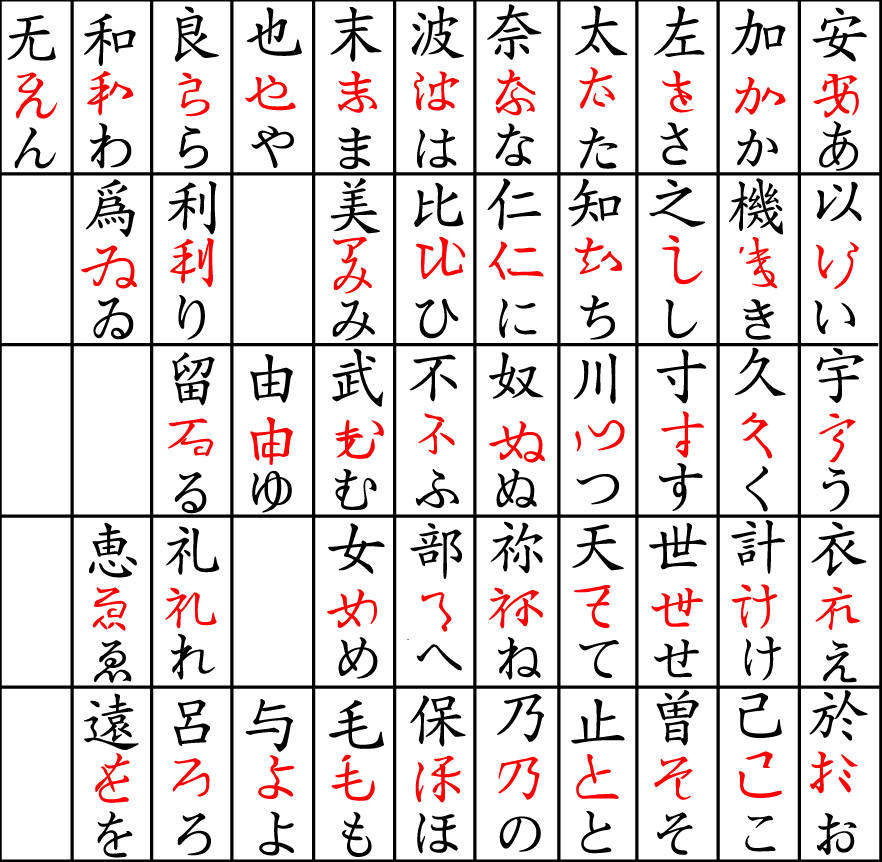
\includegraphics[width=0.8\textwidth]{Cap1/hiraganakanji}
    \caption{Adaptation from kanji to Hiragana, with the original Kanji at the top, an intermediary form in the middle and Hiragana at the bottom}
    \label{fig:kanji_to_hiragana}
\end{figure}

Prior to World War II, thousands of Kanji characters were in use in various writing systems and styles, leading to great difficulties to learning and teaching Japanese. To ease this problem, in 1946 the Japanese Ministry of Education created a list of the most commonly used 1,850 characters and declared them to be the official Kanji of the Japanese language. This list of official Kanji was called the T\={o}y\={o} Kanji (\jap{当用漢字}, literally "Chinese characters for general use"). This set of Kanji was proposed as an intermediary step for a plan that aimed at completely abolishing Kanji from the Japanese language, an ambitious plan that received strong opposition from the Japanese public.

In 1981 an updated list that added 95 additional Kanji to the T\={o}y\={o} Kanji was forwarded, and was named the J\={o}y\={o} Kanji, or Jouyou Kanji (\jap{常用漢字}, literally "Chinese characters for regular use"). In 2010 the official list was again reviewed, including additional 196 characters, while removing 5, forming the current Jouyou Kanji list with 2,136 official characters. Additionally, a second list of Kanji was created, the called Jinmeiy\={o} Kanji (\jap{人名用漢字}, literally "Chinese characters for use in personal names"). This second list supplements the Jouyou Kanji list, so that all proper names in Japanese should have all characters present in one of those two lists.

\section{Kanji Complexity Overview}\label{kanjicomplexity}

There are a number of factors that introduce complexity to the study of Japanese Kanji. Below, we list a a number of the most challenging issues.

\subsection{Various representations for the same Kanji}

For 212 Kanji in the J\={o}y\={o} Kanji there are two forms of the same character: the Old form (Ky\={u}jitai) and the Modern form (Shinjitai). Additionally, there are 4 characters listed in the Jouyou Kanji list that are not presented in Japan's basic character set, the JIS X 0208, and are thus commonly replaced by similar characters that are in this list. Therefore, in any proper statistical analysis it is required that both forms of these Kanji are mapped to the same concept. In Table \ref{tab:variants} we list 7 of these 216 variations.

\begin{table}[h]
\centering
\caption{Comparison of variants for 7 J\={o}y\={o} Kanji}
\label{tab:variants}
\begin{tabular}{|c|c|}
\hline
\textbf{\begin{tabular}[c]{@{}c@{}}New form/\\ Proper form\end{tabular}} & \textbf{\begin{tabular}[c]{@{}c@{}}Old form/\\ Adapted form\end{tabular}} \\
\hline
\Huge\jap{慎} & \Huge\jap{愼} \\ \hline
\Huge\jap{竜} & \Huge\jap{龍} \\ \hline
\Huge\jap{涼} & \Huge\jap{凉} \\ \hline
\Huge\jap{円} & \Huge\jap{圓} \\ \hline
\Huge\jap{尽} & \Huge\jap{盡} \\ \hline
\Huge\jap{礼} & \Huge\jap{禮} \\ \hline
\Huge\jap{頰} & \Huge\jap{頬} \\ \hline
\end{tabular}
\end{table}

\subsection{Multiple meanings associated to a single Kanji}
A further complication in the case of Japanese is that its roots are very apart from our own, so concepts we take as dissimilar in Romantic or Anglo-Saxonic languages may be considered to be related in Japanese, and therefore be grouped under the same ideogram. One such example is the ideogram \jap{気} that simultaneously means: spirit (as in soul), atmosphere (as in atmospheric pressure), mood/feeling, the mind and air.

\subsection{Multiple Chinese readings (on'yomi)}

As explained in Section \ref{japhistory}, the Japanese writing system was heavily influenced by Chinese. In this system, Chinese came to be the etymological root of compound words in Japanese. An analogy with the Anglo-phonic case would be the concept of Water, that can be worded as \textit{Hydro} (as in \textit{Hydraulics}) or \textit{Aqua} (as in \textit{Aquaphobia}). This kind of reading came to be known as the On'yomi. One situation that arose from this borrowing is that Chinese and Japanese use very different phonotactics. While in Japanese the only kind of different voicing is done by increasing the length of the voicing of a vowel (as in the proper name Tooru, or T\={o}ru), Chinese has five different kinds of intonations for the vowel parts of phonemes (for example: ma, m\={a}, m\`{a}, m\'{a} and m\v{a} are five different words in Chinese, differentiated solely through intonation), and also includes many consonant sounds that are not existent in Japanese. This incompatibility caused the Japanese mimics of the Chinese sound to be radically different than the original. Also, since the Chinese language entered in Japanese firstly through scholars and this was a process that lasted centuries, it occurred that miscopying was occasionally carried into Japanese as an accepted form or multiple steps of the phonetic evolution of the same word entered in Japan and multiple of those became accepted.

One such example of a Kanji with multiple on'yomi reading is \jap{数}, that represents the idea of figure or number. The officially recognized Chinese reading of this Kanji is "s\={u}", but four more readings are common: "su", "shu", "soku" and "saku". Note that the current reading in Chinese for this Ideogram is "sh\v{u}".

Figure \ref{fig:onyomihist} presents a histogram for the number of readings by Kanji. As it can be noted, most Kanji have only one Chinese reading, but about 470 have two readings and more than a hundred present three or more readings.

\begin{figure}[ht]
    \centering
    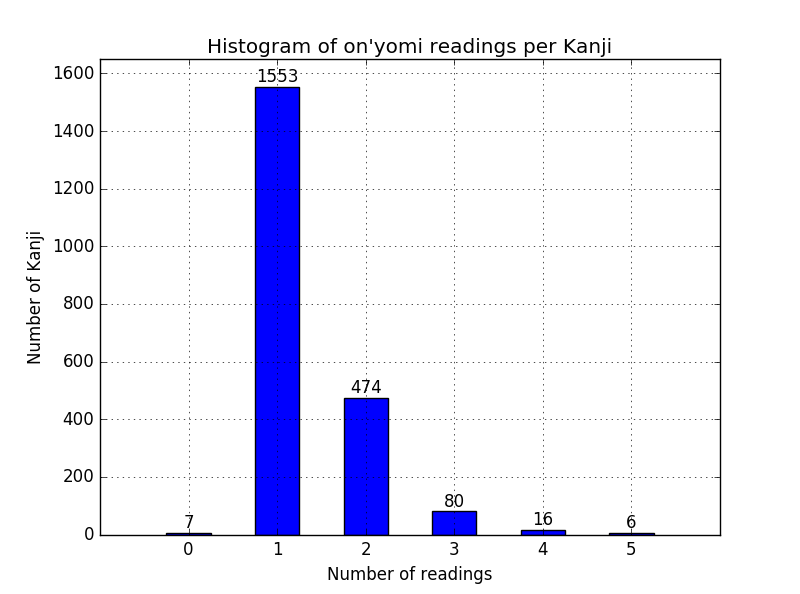
\includegraphics[width=\textwidth]{Cap1/HistogramOnYomi}
    \caption{A Histogram of the number of on'yomi readings by Kanji}
    \label{fig:onyomihist}
\end{figure}

\clearpage

\subsection{Multiple Japanese readings (kun'yomi)}

Even before the introduction of writing through Chinese influence, Japan already had a spoken language that had to be fitted to the imported characters. This kind of reading is mostly used for isolated Kanji, used as substantives, adjectives or verbs. To use again the analogy with Water/Hydro/Aqua, the kun'yomi reading would be the equivalent of the word "Water".

Once more, the Kanji \jap{数} is one that presents multiple readings. The officially recognized Japanese reading of this Kanjis are "kazu" and "kazo", though the readings "se", "wazurawa" and "shibashiba" are also used.

Figure \ref{fig:kunyomihist} presents a histogram for the number of readings by Kanji. As it can be noted, about half of the Jouyou Kanji have only one reading, but about 430 have two readings, 370 have no Japanese readings and almost 300 present three or more readings.

\begin{figure}[ht]
    \centering
    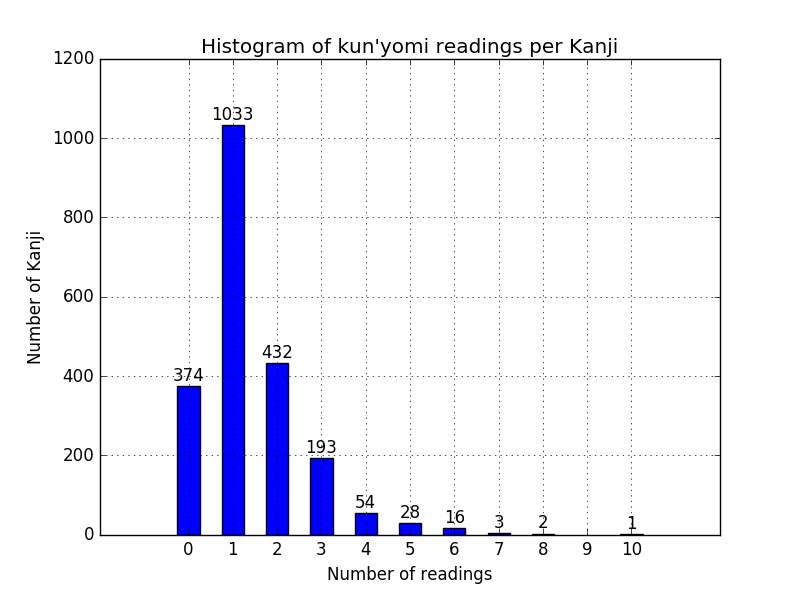
\includegraphics[width=\textwidth]{Cap1/HistogramKunYomi}
    \caption{A Histogram of the number of kun'yomi readings for Kanji}
    \label{fig:kunyomihist}
\end{figure}

\clearpage

\subsection{Readings for use in names (nanori)}

There is one more important type of reading for Kanji that should be considered by Japanese learners: the nanori reading. This type of reading represents readings for Kanji that are used in proper names (for example the name of cities, prefectures or people). 

The Kanji \jap{希}, which represents hope or request is a case with multiple nanori readings. This Kanji has the Chinese readings "ke" or "ki" and Japanese reading "mare", but in names it can be read as "nozo" or "nozomi" (note that "Nozomi" by itself is a full Japanese name).

Figure \ref{fig:nanorihist} presents a histogram for the number of readings by Kanji. As it can be noted, about 1200 Jouyou Kanji have no nanori readings, but 360 have one reading, 213 have two Japanese readings and about 350 present three or more readings.

\begin{figure}[ht]
    \centering
    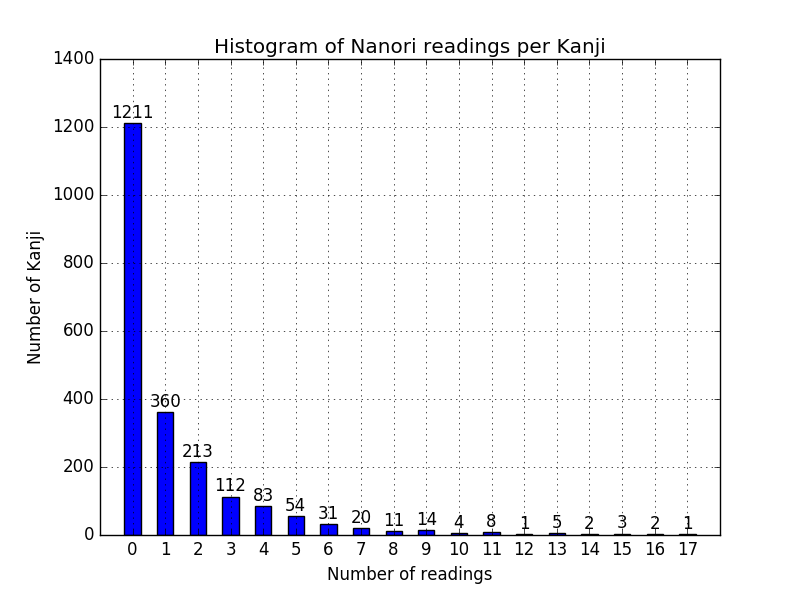
\includegraphics[width=\textwidth]{Cap1/HistogramNanori}
    \caption{A Histogram of the number of nanori readings for Kanji}
    \label{fig:nanorihist}
\end{figure}

\clearpage

\subsection{Irregular readings}

As if not enough, Kanji can also be read in a completely different fashion than its usual reading. One such example is the word \jap{一昨日} that can be read in a regular fashion as Issakujitsu (\jap{いっさくじつ}) where all parts of this word can be matched to its three ideograms: is/saku/jitsu. However, this word can also be read as Ototoi, a reading that have no connection whatsoever to the accepted Kanji readings of this word.

\subsection{Conclusion}

In brief, we can say that the task of teaching one single Kanji passes through teaching:
\begin{itemize}
    \item How this Kanji is written (including stroke order);
    \item One or more possibly dissimilar conceptual ideas to associate with it;
    \item Zero or more Chinese readings;
    \item Zero or more Japanese readings;
    \item Zero or more Naming readings;
    \item Possible words where it appear with an irregular reading;
\end{itemize}

\section{Present approaches for learning Kanji}\label{intro:presentapproaches}
A number of different methods have been proposed to teach the Japanese Kanji. For Japanese natives, the Japanese Ministry of Education have selected a list of 1,006 Kanji, the Ky\={o}iku Kanji (\jap{教育漢字}, literally the "Educational Kanji"). This list divides those 1,006 Kanji that are expected to be learnt by a native Japanese from grades one through six. Note that among Kanji of the same grade there's no order established by the Ministry of Education, and thus each school can choose the order according to its own preferences. The remaining 1,130 Kanji are expected to be studied through the three years of Junior High School. The number of Kanji that are selected for each grade is presented in Table \ref{tab:kyouiku}.

\begin{table}[ht]
\centering
\caption{Number of Kanji to be taught per grade}
\label{tab:kyouiku}
\begin{tabular}{|c|c|}
\hline
\textbf{Grade} & \textbf{Number of Kanji} \\ \hline
First & 80 \\ \hline
Second & 160 \\ \hline
Third & 200 \\ \hline
Fourth & 200 \\ \hline
Fifth & 185 \\ \hline
Sixth & 181 \\ \hline
\end{tabular}
\end{table}

This list of Kanji was developed through the combination of multiple different approaches, and do not directly reflect the frequency that these characters are present in Japanese media. Additionally, this list was put together with consideration to the age of the child in question. Considering that a First Grade child should be around 6 years old, the first grade Kanji refer to concepts that should be familiar to children that age, such as sun, moon, th ordinal numbers (1 through 10, 100 and 1,000), left, right, big, small, male and female. One example that shows how this list may not be the ideal for non-native speakers to follow is the Kanji \jap{関}, which means "to be related" or "connected". This Kanji is only taught in the fourth grade to Japanese students, but it is the 56th most common Kanji that is used in the Japanese version of Wikipedia.\footnote{This data is the result from a study made in this work, which can be found in chapter \ref{chap:frequency}.}

Another Source of order to study Japanese characters is the list that was provided by the JLPT – the Japanese Language Proficiency Test (\jap{日本語能力試験}). The organization responsible for this exam provided Kanji lists for each of its 4 levels of certificates: 103 Kanji for level four, 181 additional Kanji for level three, 739 additional for level two and finally 903 additional for level one, totalizing 1926 Kanji. Since its renewal in 2009, the JLPT became a five levels exam and stopped providing Kanji list. Since those official lists take in consideration non-native Japanese students, it is still a widely used guide to the order of Kanji to be learnt, although no order withing this levels was predetermined by the JLTP organization.

With this and other issues presented in section \ref{kanjicomplexity}, it is evident that non-native speakers can benefit much with learning media that are targeted specifically to their needs. Below are listed a number of different media that seeks to teach Japanese Kanji to non-native speakers, each followed by a critique of pros and cons.

\subsection{Learning Books}

\subsubsection{Kanji Look and Learn}

Kanji Look and Learn\cite{kanjilookandlearn} is a book by a collaboration of 5 Japanese teachers and is one of the most famous books for learning Japanese Kanji. In fact, it is a series of books that divides Kanji according to its grade on the previous lists issued by the JLPT organization. Figure \ref{fig:lookandlearn} presents the book cover and a small excerpt of the book.

\begin{figure}[ht]
    \begin{subfigure}{0.5\textwidth}
    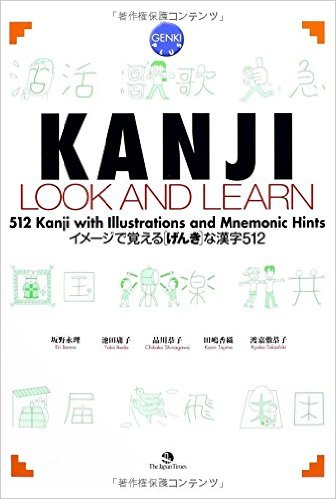
\includegraphics[width=0.9\linewidth]{Cap1/LookAndLearnKanji}
    \caption{Cover of Kanji Look and Learn.}
    \label{fig:lookandlearncover}
    \end{subfigure}
    \begin{subfigure}{0.5\textwidth}
    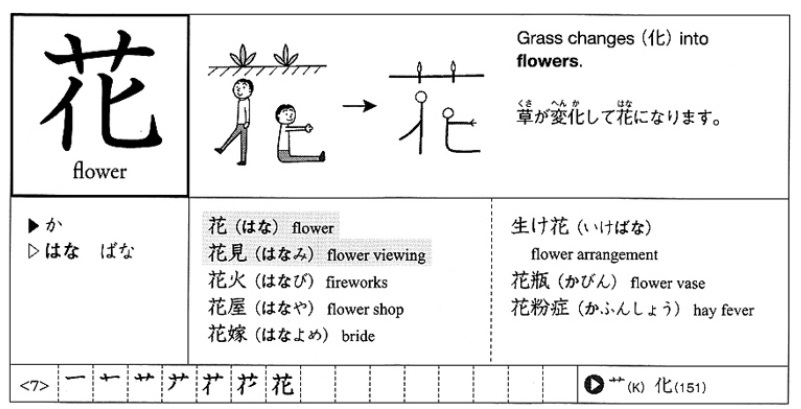
\includegraphics[width=0.9\linewidth]{Cap1/LookAndLearnPage}
    \caption{Excerpt from the book.}
    \label{fig:lookandlearnpage}
    \end{subfigure}
    \caption{Cover and Excerpt from Kanji Look and Learn.}
    \label{fig:lookandlearn}
\end{figure}

Like all the other examples of this section, this is a great book. Some advantages it has are:
\begin{itemize}
    \item Shows visual representations for Kanji using real life objects;
    \item Shows Japanese and Chinese readings;
    \item Presents multiple examples per Kanji;
    \item Displays stroke order;
    \item Separates Kanji among morphological radical parts;
    \item It has a simple clean interface for each Kanji;
\end{itemize}

Some limitations it faces are:
\begin{itemize}
    \item As any book, finding an information can be hard, encouraging a passive form of study (indexing problem);
    \item No Nanori readings are presented;
    \item Just a small number of Japanese and Chinese readings are presented;
    \item Even if radicals are broken up, it is hard to answer simple questions as "which other Kanji shares this same radical" or "is this Kanji visually similar to any other Kanji" or "is this Kanji a sub-component of any other Kanji";
    \item Definitions for words are short, making it possibly hard to understand the concept;
    \item Example words are not sorted by frequency, and a relatively small number of examples is shown;
\end{itemize}

\subsubsection{A guide to Remembering Japanese Kanji}

This Kanji study book by Kenneth G. Henshall\cite{henshall1988guide} is a classic and takes a very different approach to most other books. Firstly it develops from a serious and well structured history research that tries to uncover the true formation factors of the Kanji. It presents Kanji by the order established for grades in the Ky\={o}iku Kanji, and sorts Kanji alphabetically through their Chinese readings. Figure \ref{fig:henshallbook} presents the book cover and a small excerpt.

\begin{figure}[ht]
    \begin{subfigure}{0.5\textwidth}
    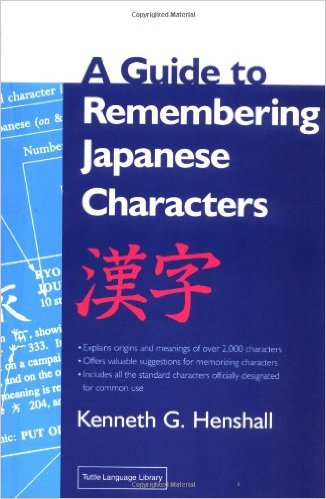
\includegraphics[width=0.9\linewidth]{Cap1/AGuideJapaneseCover}
    \caption{Cover of A Guide to Remembering Japanese Characters.}
    \label{fig:henshallbookcover}
    \end{subfigure}
    \begin{subfigure}{0.5\textwidth}
    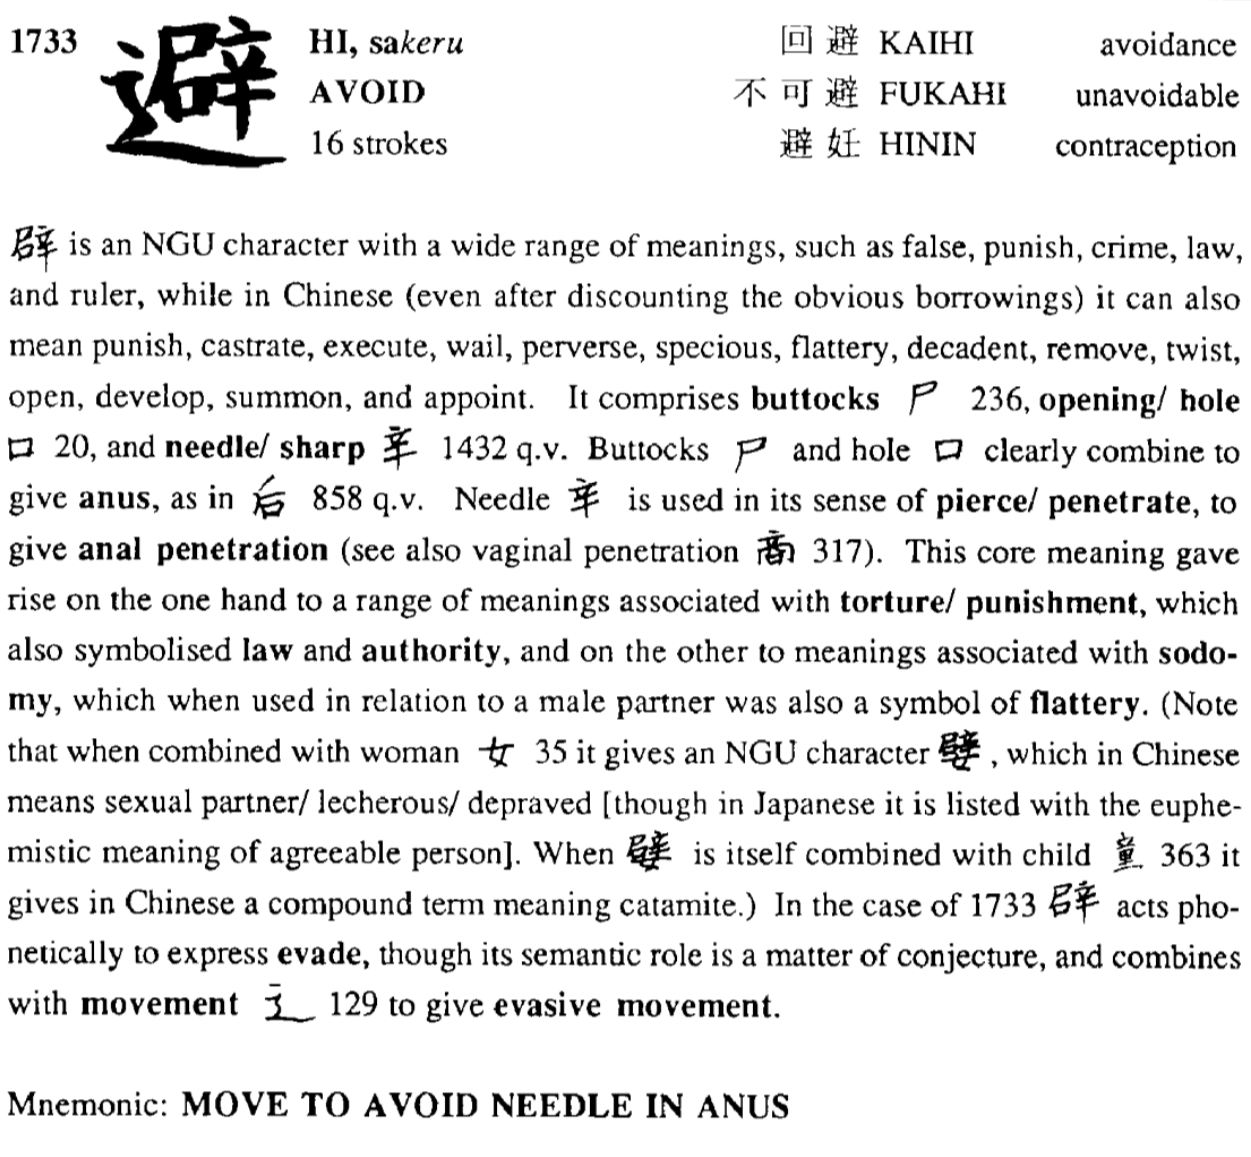
\includegraphics[width=0.9\linewidth]{Cap1/AGuideJapanese}
    \caption{Excerpt from the book.}
    \label{fig:henshallbookpage}
    \end{subfigure}
    \caption{Cover and Excerpt from A Guide to Remembering Japanese Characters.}
    \label{fig:henshallbook}
\end{figure}

Some advantages it has are:
\begin{itemize}
    \item Presents a very accurate description of the character morphological history, also defining which of its radicals are thought to have phonetic influence and which are thought to have conceptual influence;
    \item Shows On and Kun readings;
    \item Displays stroke number;
    \item Presents example words;
    \item Presents a mnemonic;
    \item Numbers Kanji in a fashion that is recognized by other important Japanese learning media, making it easy to refer to this book from ;
    \item cross references Kanji with other information that can be looked up through entry numbers;
\end{itemize}

Some limitations it faces are:
\begin{itemize}
    \item Once again, it presents indexing problems for looking up Kanji and relations between multiple Kanji;
    \item No Nanori readings are presented;
    \item Just a small number of Japanese and Chinese readings are presented;
    \item Does not always breaks a Kanji in its radical components;
    \item Definitions for words are short, making it possibly hard to understand the concept;
    \item Example words are not sorted by frequency, and a relatively small number of examples is shown;
    \item A great number of Kanji have very obscure history, provided that many of these have millennium of history, making this kind of study frustrating at times;
    \item Each entry presents a great deal of information which can not be minimized to browse only the essential pieces of information and connections;
\end{itemize}

\subsection{Websites}

\subsubsection{Jisho.org}

The Denshi Jisho project\cite{jishoorg} describes itself as: "Jisho is a powerful Japanese-English dictionary. It lets you find words, Kanji, example sentences and more quickly and easily". It is a free and open project that serves many functions, being in essence a very powerful and clean interactive dictionary in English for the Japanese language. As written in the website footnote, it was "lovingly crafted by Kim, Miwa and Andrew". Figure \ref{fig:jisho} presents an example entry of the Kanji dictionary functionality of this website.

\begin{figure}[ht]
    \centering
    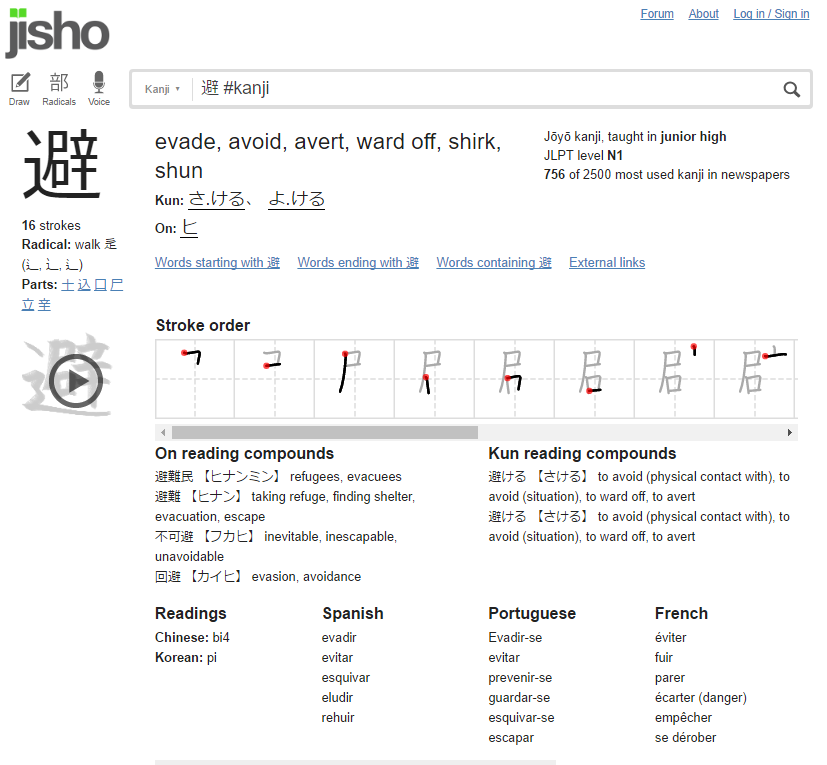
\includegraphics[width=0.8\textwidth]{Cap1/DenshiJisho}
    \caption{An example entry from Jisho.org}
    \label{fig:jisho}
\end{figure}

\begin{figure}[ht]
    \centering
    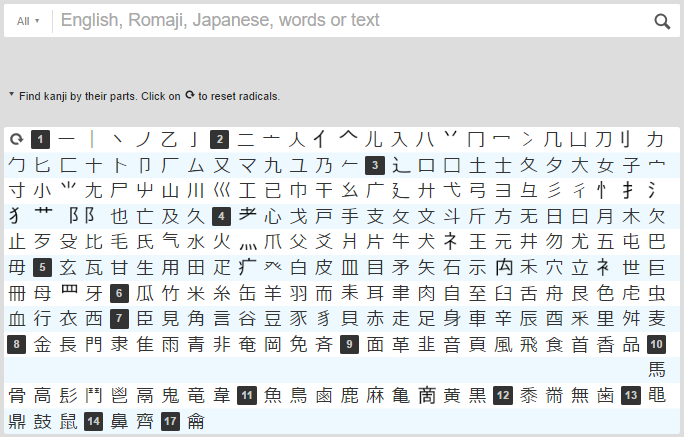
\includegraphics[width=0.5\textwidth]{Cap1/RadicalSearch}
    \caption{Radical look-up feature from jisho.org}
    \label{fig:jishoradsearch}
\end{figure}

It is a very useful website and has the following perceived advantages:
\begin{itemize}
    \item It has a very complete search capability, being able to look for Kanji from hand drawings, its radical parts (refer to figure \ref{fig:jishoradsearch}) and even through voice;
    \item Presents multiple links that can be followed for more information about a part, including some component parts;
    \item Provides a very complete set of definitions each Kanji can assume;
    \item Separates examples were it can be seen with its Chinese and Japanese Readings;
    \item Presents Nanori readings, when they exist;
    \item Displays definitions in multiple languages;
    \item Has animated and step by step stroke order guides;
    \item Displays information of frequency, JLPT level and Ky\={o}iku grade;
    \item It is free, which increases its reach;
\end{itemize}

Unfortunately, it has a few shortcomings:
\begin{itemize}
    \item The list of parts it is composed of is confusing, and does not follow any clear rule;
    \item Does not present simple relationships among characters, like which characters are composed of which other Kanji. For example, the Kanji in figure \ref{fig:jisho} is \jap{避} and has one big component that is not shown in Jisho's list: \chin{辟}. The provided list falls somewhat between trying to show all components to showing some that are apparently disconnected from this Kanji (such as \jap{込}). Following through the analysis of \chin{辟}, we note that it appears in four and four only J\={o}y\={o} Kanji: \jap{避}, \jap{璧}, \jap{壁}, \jap{癖}. This relationship cannot be attained in any easy way from Jisho's website, since the radical \chin{辟} is not one of its supported at its radical look-up screen (refer to figure \ref{fig:jishoradsearch}) either;
    \item Does not have a learning platform, only a browsing feature;
    \item Does not present a feature where characters are listed in ascending or descending order with their frequency;
\end{itemize}

\subsubsection{Wani-Kani}

Wani-Kani\cite{wanikani} is a paid web-app from where the "parts" and radicals used in Jisho.org were granted. It has a very complete learning feature, with a dedicated team to hand proof its data and designers to make elaborate custom mnemonic drawings. Its merits, according to its own description, are listed in figure \ref{fig:wanikani} and also explained below.

\begin{figure}[ht]
    \centering
    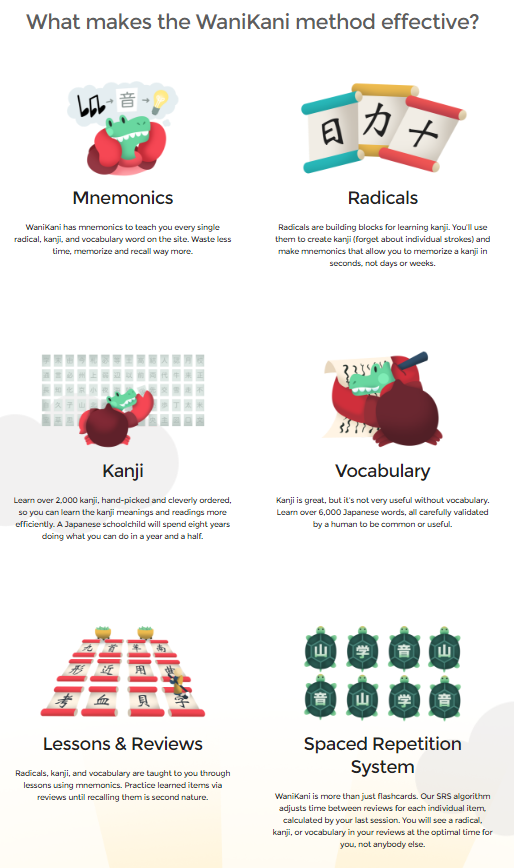
\includegraphics[width=0.8\textwidth]{Cap1/WaniKani}
    \caption{Wani-Kani advertised advantages}
    \label{fig:wanikani}
\end{figure}

\begin{itemize}
    \item Mnemonics: Has one mnemonic for every Kanji;
    \item Radicals: Approaches every Kanji from a building perspective, always teaching radicals prior to a Kanji;
    \item Kanji: Attempts to teach all 2,136 Jouyou Kanji, in a way that is "cleverly ordered";
    \item Vocabulary: It uses example words, as all previous books;
    \item Lessons \& Reviews: The website does not provide a browse feature (at least not until a character is considered to be learned), but only a Lessons and Reviews board;
    \item Spaced Repetition System: uses SRS theory\cite{baturay2009effects} to make spacing custom to each student;
\end{itemize}

Although all of these and other merits can rightfully be associated with Wani-Kani, it also has a number of perceived issues:

\begin{itemize}
    \item It is a paid service, which curbs its access rate and therefore its teaching potential;
    \item The website does not adapt well to its user preferences. For example: there is no functionality that lets the user edit and choose its own mnemonics in favor of those proposed unilaterally by Wani-Kani;
    \item Radicals are not well separated from Kanji, and the approach this website use to define which are the components of a Kanji (a process that is not always so straightforward) is not clear, sometimes referring to radicals for their visual appearance (As Kanji Look and Learn does) and some times for technical correctness (as Henshsall's Guide does);
    \item The "cleverly ordered" form does not follow any apparent technical guideline, just humans' subjective opinions;
    \item Shows a very limited number of words for each Kanji (a mean of three).
    \item Does not provide a leveling method, following the same bottom-up approach for every student;
    \item Its system does not facilitate browsing through Kanji, nor does it show important relations also missing from Jisho.org;
    \item Its Spaced Repetition System algorithm appears to treat Kanji as independent learning subjects, when in fact they have very rich relational structures among themselves;
\end{itemize}


\clearpage

\section{The need for a new way of learning}\label{intro:newway}

Taking in consideration all the advantages and disadvantages listed for the provided examples, we clearly notice that a new way of learning would greatly benefit Japanese learners. Firstly, this new way of learning should be a website, since it inherently holds many advantages in comparison with books, such as a bigger space for information, interactivity, indexing functions, browse and learning aids. 

On a second note, it can be noted that Jisho.org and Wani-Kani are already great learning aids, but each of them still holds some limitations. The work developed in this Academic Work is a stepping stone in the direction of creating a website that takes advantages of most of the functions that are considered to be advantages on those two platforms, as well as addressing their shortcomings.

Chapter \ref{chap:frequency} elaborates on the issue of taking Kanji frequency in Japanese media more seriously, so that the a student can have maximum success in learning frequent Kanji in minimal time.

% Chapter \ref{chap:readings} describes work in the direction of automatically matching Kanji readings to example words for a large number of those, also making associations of the Kanji to a Compiler Grammar.

Chapter \ref{chap:graphs} elaborates the concept of teaching order further, elaborating two graphs that relate Kanji among themselves (a morphological graph and a co-occurrence graph), as well as providing predictions of behaviors of students in analogy with random walk models with random restarts. 


Finally, Chapter \ref{chap:teaching} uses the knowledge obtained in previous chapters to propose specific details of the future website functionality in order to create an efficient teaching aid for the study of Japanese Kanji.

\chapter{Linguistic Frequency Distribution}
As explained in section \ref{intro:newway} of the introduction chapter, one aspect that deserves special attention when teaching Japanese is the \textbf{importance} of a word or Kanji. Importance can be defined in a number of ways, such as the definition implied by the grade lists brought forward by the Japanese Ministry of Education, the Ky\={o}iku Kanji, which were introduced at section \ref{intro:presentapproaches}. This grading system uses a constructivist approach, where Kanji that hold more simple and concrete meaning are taught earlier than Kanji that represent more complex or abstract ideas. Additionally, the Ky\={o}iku Kanji grades also reflect the frequency which characters are expected to be present in text compatible with the age of the student in question\footnote{For example, a student learning first grade Kanji should be around six years old, and therefore be presented more often with text where the concepts, and therefore the Kanji, are simple}.
Although this specific order proves itself useful when teaching native Japanese children, it is not necessarily the best order to teach foreign adults that are seeking to learn Japanese as an additional language.

Taking these cases in mind, we propose that for adults, a much more concerning factor in deciding which Kanji should be tackled first and with more seriousness\footnote{In here, we assume that the study technique will be similar to a factorial method: the student will learn one topic and progress to learn other topics returning from time to time to check if the first concepts are clear. If this is the method used in a web app to teach Japanese, the first Kanji to be taught would also coincide with those that are expected to be the best understood} would be the relative frequency this Kanji is used in media that he is likely to be interested in. It is important to note that the order proposed in this chapter is not the final order that would be advised to be used in the study of Japanese Kanji, but only a stepping stone in the direction of obtaining this better list. Chapter \ref{chap:graphs} elaborates more on other factors that should be considered when estimating the importance of a Kanji character.

In the next sections, we describe the process of seeking an appropriate source of data, we compare the total word distribution and Kanji-only distribution to a power log distribution (also known as Zipf's distribution) and finally we explore the implications of the relationship of the specific format of the frequency distribution curves and the learning process of a student.

\section{Frequency estimation of Japanese text}
Japanese has a number of particularities that make the frequency estimation of words (or lemmas) to be unique, and should be explained in order to understand the complexity and steps of the process.

\subsection{Parsing the Japanese Language}\label{freq:parsing}
The Japanese language does not use the concept of blank spaces in its writing system, although it does use some punctuation marks such as commas, periods and exclamation marks. That being so, the task of reading Japanese also comprises the task of determining the start and end of words and syntax particles.
As an example, let us examine a simple sentence in Japanese: The cat is sitting on the roof.

\begin{center}
\jap{猫が屋根に座っている}
\end{center}

Firstly, it can be noted that there are ten graphemes in this sentence, but no spacing marks, as mentioned earlier. Now, let us artificially introduce space marks along with a r\={o}maji transliteration\footnote{refer to Section \ref{ape:romanization} in the Appendix for more information about the romanization process} below.

\begin{center}
\jap{猫 が 屋根 に 座っている}\\
neko ga yane ni suwatteiru
\end{center}

With this, we identify five separate words in this sentence. It was possible to do the parsing of this sentence due to the previous knowledge of the structure of Japanese sentences and the function each word plays in the sentence. Initially we read the Kanji \jap{猫}, which is read as neko and means "cat", we identify this as an individual word of the sentence and expect the next element to be a syntax particle, designing the function of this element in the sentence. In succession, we find the Hiragana \jap{が}, ga, the subject marker, which indicates that "cat" is the subject. We then proceed to look for the predicate of this sentence and find the word with two Kanji \jap{屋根}, yane, which means "roof". We then expect to see a direct or indirect object particle marker, and thus we find the Hiragana \jap{に}, ni, the indirect object marker. Finally we expect to find the verb of the sentence
\footnote{Japanese is structured around Subject/Object/Verb, instead of the form Subject/Verb/Object, which is more common in western languages}, 
and read the Kanji accompanied by some Hiragana stem \jap{座っている}, suwatteiru, the verb "to sit" in the present progressive form.

This task of identifying word boundaries is much facilitated by the intermixing of Kanji, Hiragana and occasionally Katakana in sentences, which is one of the reasons that makes Kanji so useful for the Japanese language.

\subsection{Lemma extraction (optional)}

Optionally, the occurrence of elements can be done around lemmas instead of words. Lemmas are the unification of multiple words under a same root such as the uninflected forms of words. With this process, different representations of the same concept can be condensed to a unique entry, instead of having it spread in multiple entries. In English the process would be similar to unifying the words \textit{"moves"}, \textit{"moving"} and \textit{"moved"} to the word \textit{"move"}. Figure \ref{fig:lemmas} exemplifies the process in English and Japanese. In the case of the Japanese language there's an additional issue that may be solved, which is the unification of homographs under a same lemma. For example, both spellings \jap{お勧め} and \jap{お薦め} are valid ways to write \jap{おすすめ}, osusume, which means recommendation.

\begin{figure}[ht]
    \begin{subfigure}{0.5\textwidth}
    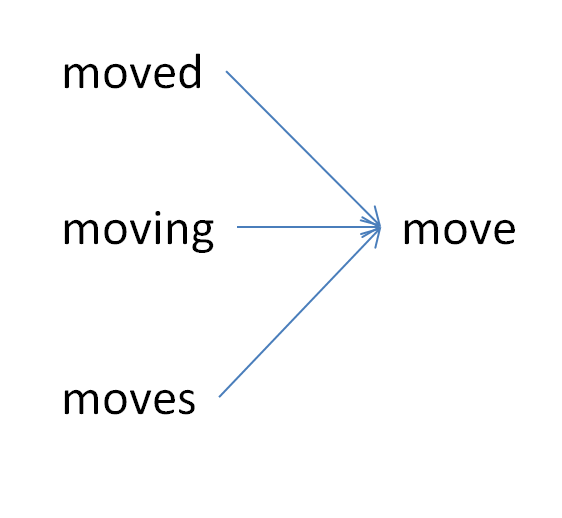
\includegraphics[width=0.9\linewidth]{Cap2/LemmaEnglish}
    \caption{Lemma extraction in English.}
    \label{fig:lemmaeng}
    \end{subfigure}
    \begin{subfigure}{0.5\textwidth}
    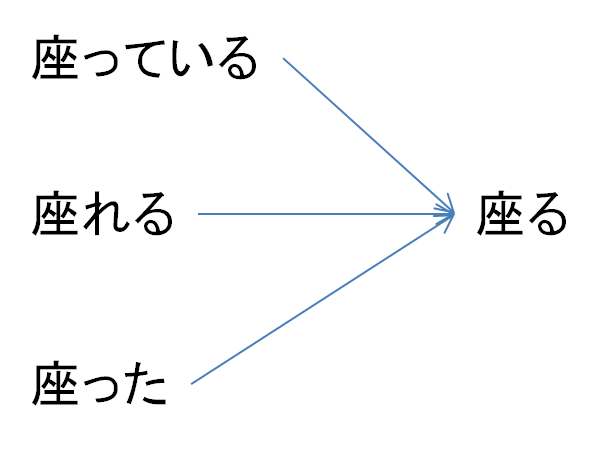
\includegraphics[width=0.9\linewidth]{Cap2/LemmaJapanese}
    \caption{Lemma extraction in Japanese.}
    \label{fig:lemmajap}
    \end{subfigure}
    \caption{Comparison of lemma extraction in English and Japanese.}
    \label{fig:lemmas}
\end{figure}

\section{Projects that estimate word frequencies}
A variety of different projects undertake the mission of determining which are the most common words in the Japanese Language. Each of the next three presented projects were taken from a different type of media.

\subsection{Alexandre Girardi's analysis of newspaper data}
This is the oldest of the three projects, dating to 1998, and was taken from parsing 4 years of the newspaper Mainichi Shinbun (\jap{毎日新聞}, literally "Daily Newspaper"), in a total of 74,721,217 occurrences spread among 311,049 words\cite{monash}. This is the most widely used project when estimating Kanji frequency rank, since this rank is already in built in a number of open source projects, including the most widely used open-source dictionary of Japanese words, Jim Breen's WWWJDIC\cite{breen2000japanese}. Alexandre Girardi's project has four main problems: first, the fact that the type of speech used in newspapers in Japanese is radically dissociated from the common day-to-day written form of Japanese. A second issue is that it is skewed to some few topics, such as economy, politics and weather forecast. The third issue is that this project is based around word extraction, instead of lemma extraction. Finally, a fourth issue is that the methodology used in this project was not clearly published by Alexandre Girardi, limiting itself to some few lines in a readme file.

\subsection{Wikitionary analysis of a Japanese Wikipedia dump}
The project in question was drawn from a complete dump of the Japanese Wikipedia on April 22th, 2015, using the morphological analyzer MeCab\cite{kudo2005mecab} and cleaning the end results to unify words under lemmas, yielding a total of 669,419,716 occurrences spread among 2,610,776 lemmas\cite{wikitionary2015wordfreq}. It is important to note that a great number of lemmas appears only one or two times. A great number of this rare lemmas are attributable to Hiragana transliterations of Kanji words inside parenthesis, a phenomena that is customary for the first sentence of each article. For example, the article about the Japanese language starts with:

\begin{center}
\jap{日本語(にほんご、にっぽんご)は、}
\end{center}

As we can see, this article starts by writing "Japanese Language" in Kanji, followed by two different possible readings for this word. In this case, since a sequence of Hiragana can be usually converted to a number of different words with different meanings, the lemma extraction failed to unify these with the lemmas containing Kanji.

If we limit the examples only to lemmas that appear more than once, the total number of occurrences is reduced to 668,024,047 occurrences over 1,214,107 lemmas. If we limit to only lemmas with at least three samples, the total number of occurrences is then reduced to 667,301,019 occurrences over 853,593 lemmas. As it can be noted, each step in this direction reduces the total number of occurrences by only a small fraction, while the number of words drops quickly in comparison with its scale. This project can be seen as as improvement over Alexandre Girardi's project for its sheer size (over 669 million \textbf{lemmas} occurrences on this project, while the previous one was resumed to only 74 million \textbf{words} occurrences) and the fact that it does lemma unification. However, the written form usually used in Wikipedia is also of a different sort than the form of speech that would be more expected to see in day-to-day texts for its formality, and it also presents a imbalance of terms, this time toward date related Kanji (the Kanji for year is specially oversampled), as well as descriptive terms. Also, simple concepts such as the Kanji for "ear" and other very simple Kanji are specially undersampled, since they represent simple concepts that are not useful in explaining other concepts.

\subsection{Christopher Brochtrup's analysis of Japanese novels}
In 2007, Christopher Brochtrup created a tool called the "Japanese Text Analysis Tool"\cite{christopher2007tool}, for the analysis of arbitrary Japanese texts, including an inbuilt capability of doing morphological parsing of texts through the MeCab\cite{kudo2005mecab} analyser followed by a word frequency report, along with other functionalities. To present as an example of this tool, on May 27th, 2012, he created a report from 5000+ Japanese novels that were in public domain\cite{christopher2007wordfreq}. This analysis was done by lemma reduction to root forms of conjugated words, but with no attempt to unify different spellings of words under one type of writing. This analysis counted a total of 366,120,879 occurrences, spread over 193,121 lemmas. It is a matter of course that this project also shows an imbalance toward words more commonly used in novels, but a comparative analysis of Kanji rank versus Japanese grade did not show any significant problems. As for its size, it is composed of almost 5 times the number of occurrences in the newspaper data and about half the number of occurrences of the Wikipedia project. These are spread over only 193 thousand lemmas, a number much more closely related to the expected size of a language vocabulary.

\subsection{Final choice and considerations}
Each of the presented projects have its own implementation and data-cleaning process particularities, but all of them fall victim to the same shortcoming: being single-sourced.

The relative frequency of words holds a strong dependence with the media at which it is published in. That being the case, the most appropriate choice would be taking multiple sources and conjoining them in a manner as to respect their individual scale of total words and to keep the statistical properties of each project, also adjusting each to be centered around the same lemma creating strategy, instead of a word-listing fashion. An even greater enhancement would be aggregating even more sources of data, and classifying those in respect of topics, interests and expected readers age group, so that a different frequency distribution could be generated for each class of user profile, specifically tailored to that profile's tastes and needs.

Since this task of pluralizing the sources of data was considered to be outside the scope of this academic work, it was not executed and is proposed as a possible improvement over the results presented in this work. Instead, we choose the media that was the most expected to be useful to an adult learner with broad interests: \textbf{we choose to use Christopher Brochtrup's analysis of Japanese novels}. That being the case, we will be optimizing the learning experience of a student that tries to read Japanese novels. It is important to note that since this decision was in some sense arbitrary and therefore may be expected to change in a future step of this project, the back-end of the analysis framework developed was designed in a way that does not make any assumptions about the origin of the lemma-count pairs, so that this source could be easily replaced with any other project that provides words in the format "count,word(or lemma)" in a .csv file.

\section{Zipf's Law}
The Zipf law is an empirical law that states that given the evolution of a natural language, the frequency of any given word is approximately proportional to its rank in a biggest-to-lowest frequency table, a rule also known as the power law. It is generally recognized as so since it was popularized by the American linguist George Kingsley Zipf\cite{zipf1935psycho}. His work comprised a hand counting and later on a log-log analysis of James Joyce's book Ulysses. Zipf noticed that in this graph the series of points seemed to from an apparent downward straight line, giving rise to the law enunciated above, or in a more technical fashion in equation \ref{eq:zipf}.

\begin{equation}\label{eq:zipf}
    f(r)\propto1/r^\alpha
\end{equation}

Where \(\alpha \approx 1\). A generalization of this law that more closely fits the frequency distribution in languages was proposed by Mandelbrot\cite{mandelbrot1962paretian}, and is expressed in equation \ref{eq:mandel}.

\begin{equation}\label{eq:mandel}
    f(r)\propto1/(r+\beta)^\alpha
\end{equation}

Where \(\alpha \approx 1\) and \(\beta \approx 2.7\). While the original equation portrays a perfectly straight line in the log-log graph, the Zipf-Mandelbrot equation yields a downward facing curve formed by the connection of two approximately straight lines. The behaviour of this \(\beta\) parameter is exemplified in figure \ref{fig:mandelbrotbeta}.

\begin{figure}[ht]
    \centering
    \begin{subfigure}{0.475\textwidth}
    \centering
    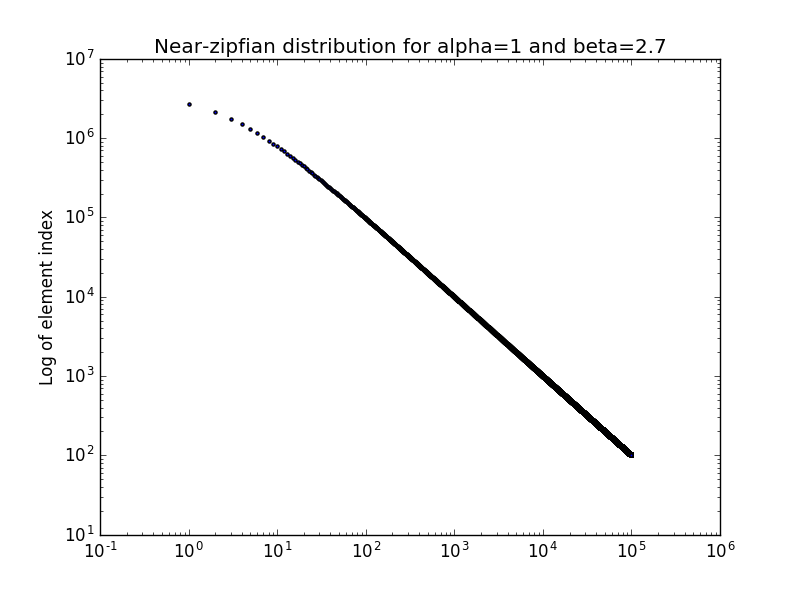
\includegraphics[width=0.9\linewidth]{Cap2/zipf27}
    \caption{Using \(\beta = 2.7\).}
    \label{fig:zipf27}
    \end{subfigure}
    \begin{subfigure}{0.475\textwidth}
    \centering
    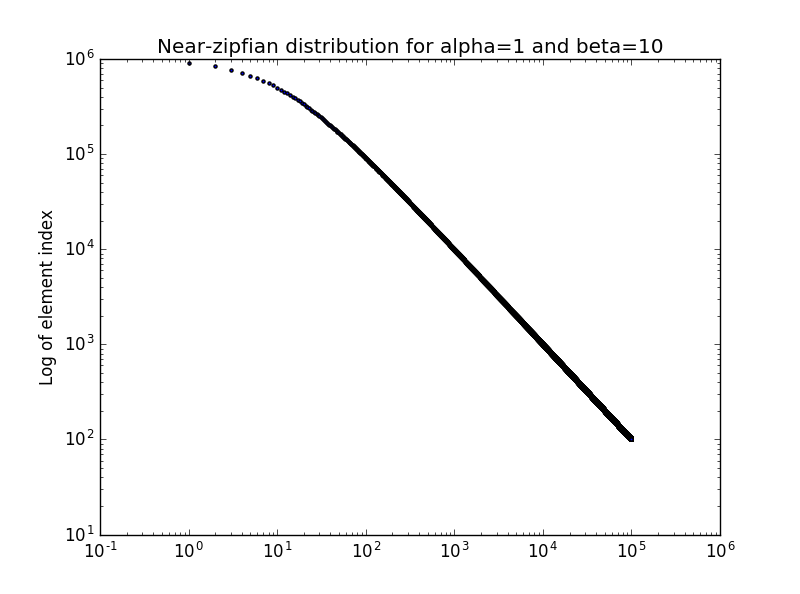
\includegraphics[width=0.9\linewidth]{Cap2/zipf10}
    \caption{Using \(\beta = 10\).}
    \label{fig:zipf10}
    \end{subfigure}
    
    \begin{subfigure}{0.475\textwidth}
    \centering
    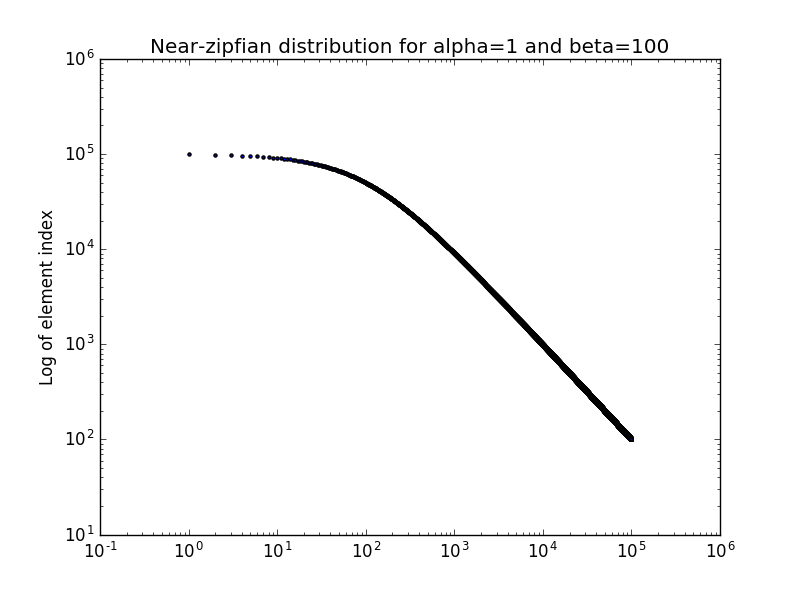
\includegraphics[width=0.9\linewidth]{Cap2/zipf100}
    \caption{Using \(\beta = 100\).}
    \label{fig:zipf100}
    \end{subfigure}
    \begin{subfigure}{0.475\textwidth}
    \centering
    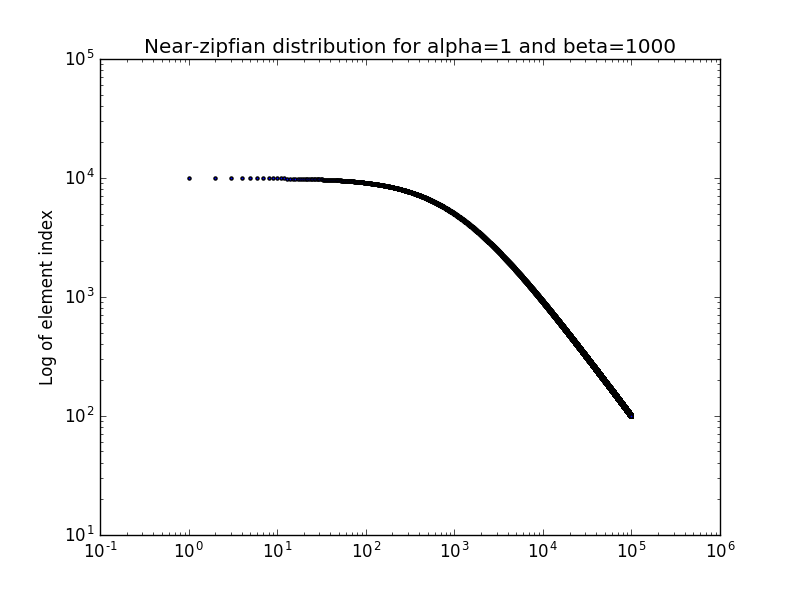
\includegraphics[width=0.9\linewidth]{Cap2/zipf1000}
    \caption{Using \(\beta = 1000\).}
    \label{fig:zipf1000}
    \end{subfigure}
    
    \caption{Log-Log graphs of data produced according to Zipf-Mandelbrot equation with various parameters.}
    \label{fig:mandelbrotbeta}
\end{figure}

As it can be seen in this sequence of four figures, as the parameter beta increases the fall of the curve is delayed.

Although a number of possible explanations were given about the origin of this phenomena, with a number of different deductions from base principles arriving at this same formula, very few of these theories focus themselves in giving testable accounts of which should be the right theory for the psychological mechanisms responsible for this effect\cite{piantadosi2014zipf}. 

In the subsequent sections we will analyse a number of frequency distribution and will do various analysis of the shape of the Log-Log graphs of these distributions. Although a more rigorous scrutiny over the presence of absence of power log behaviour would be possible through mathematical tools\cite{newman2005power}, we will focus on a simple visual analysis of the curve, giving more emphasis to the basic insights that these can bring.

\section{General Word Distribution}\label{freq:word}

Using Christopher Brochtrup report, the process of creating a \(occurrence \times rank\) graph is very straight forward. We simply produce the scatter plot of the occurrence of lemmas versus their rank in a sorted list where their counts are decreasing with the increase of their rank. The result of this analysis on linear and log-log scale is presented on Figure \ref{fig:lemmacount}.

\begin{figure}[ht]
    \centering
    \begin{subfigure}{0.475\textwidth}
    \centering
    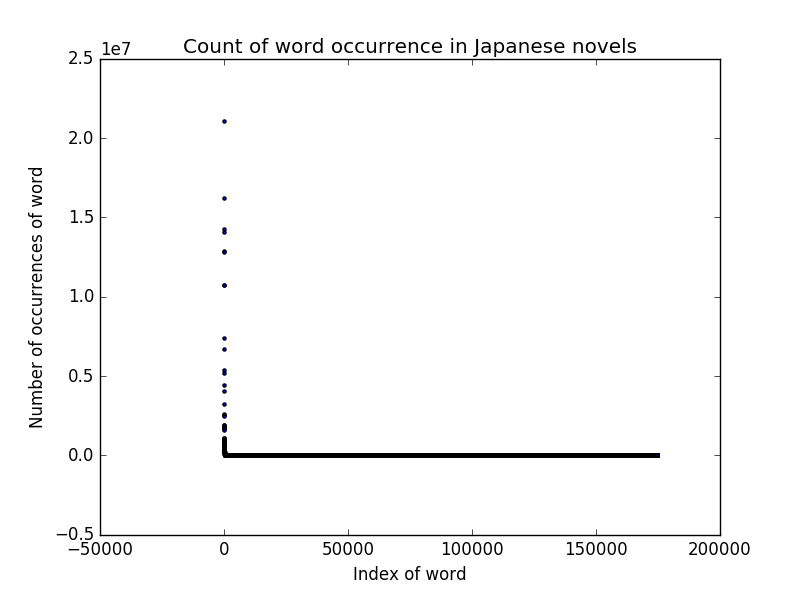
\includegraphics[width=0.9\linewidth]{Cap2/WordCountNovels}
    \caption{Linear distribution of lemmas.}
    \label{fig:lemmalinear}
    \end{subfigure}
    \begin{subfigure}{0.475\textwidth}
    \centering
    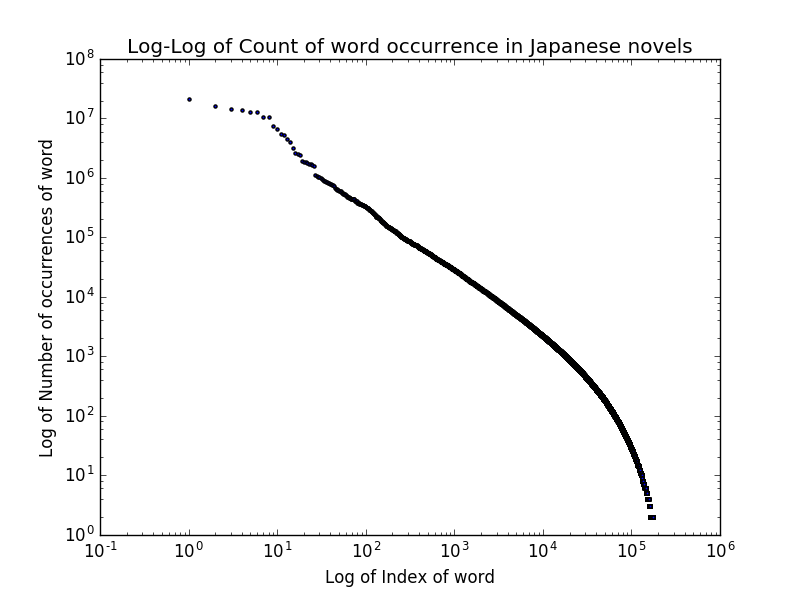
\includegraphics[width=0.9\linewidth]{Cap2/LogLogWordCountNovels}
    \caption{Log-Log of the distribution of lemmas.}
    \label{fig:lemmalog}
    \end{subfigure}
    
    \caption{Distribution of lemmas used in Japanese Novels.}
    \label{fig:lemmacount}
\end{figure}

The linear graph does not bring much insight except for the expected fact that the first few words appear a lot, with a long tail of lemmas that only happen a few times. Upon inspection of the Log-Log graph, we are able to more concretely grasp the exchange rate between the rise of the index and the fall of the number of occurrences of words takes place. In this case, we can visually detect that the curve has a Near-Zipfian behaviour, with most of the core part of the curve closely matching a straight curve. This was to be expected, since most human languages were already observed to be closely related to power log curves.

\section{Distribution of Words with Kanji}\label{freq:wordwithkanji}

We can now refine our earlier data-set so that it is exclusively formed by words with at least one J\={o}y\={o} Kanji, keeping the ordering as was done in the previous section. The result of this analysis is presented in Figure \ref{fig:lemmacountwkanji}.

\begin{figure}[ht]
    \centering
    \begin{subfigure}{0.475\textwidth}
    \centering
    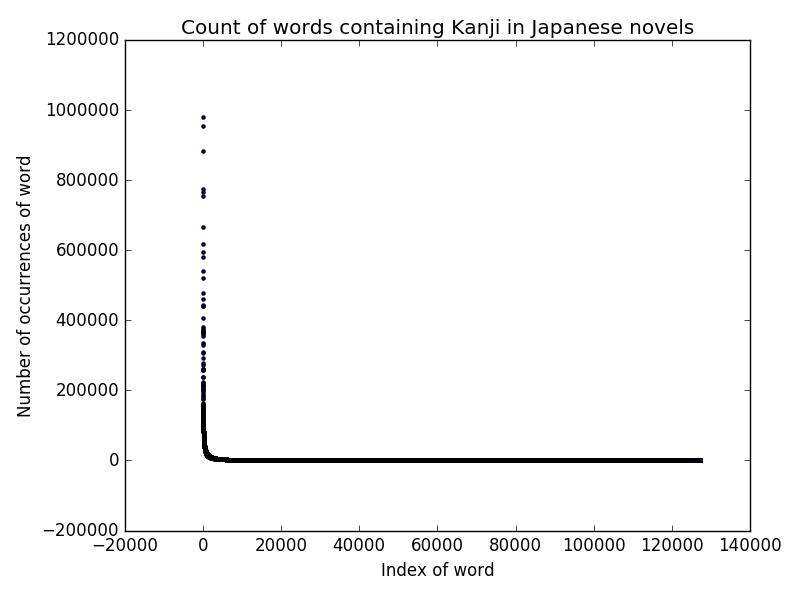
\includegraphics[width=0.9\linewidth]{Cap2/WordCountWithKanjiNovels}
    \caption{Linear distribution of lemmas.}
    \label{fig:lemmalinearwkanji}
    \end{subfigure}
    \begin{subfigure}{0.475\textwidth}
    \centering
    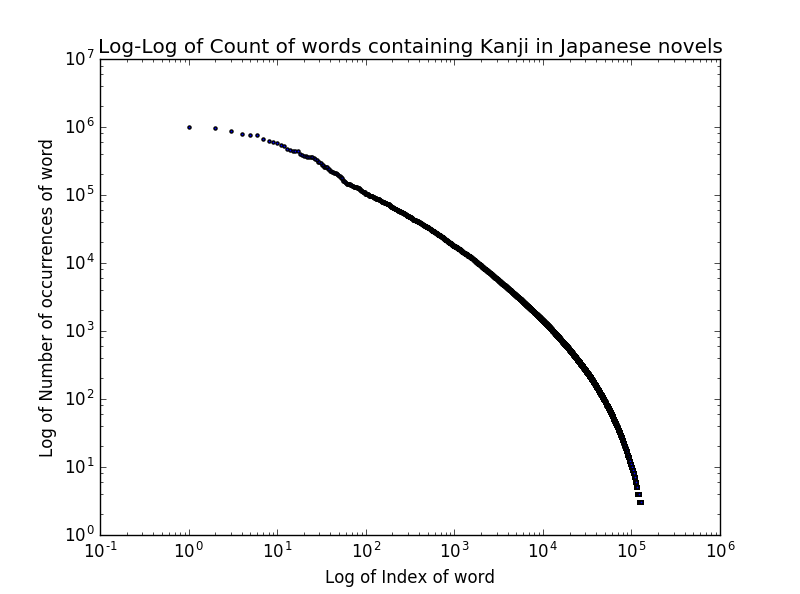
\includegraphics[width=0.9\linewidth]{Cap2/LogLogWordCountWithKanjiNovels}
    \caption{Log-Log of the distribution of lemmas.}
    \label{fig:lemmalogwkanji}
    \end{subfigure}
    
    \caption{Distribution of lemmas used in Japanese Novels that contain at least on Jouyou Kanji character.}
    \label{fig:lemmacountwkanji}
\end{figure}

Once again, we note that the linear plot is only able to bring the expected insight that the occurrences of lemmas are highly concentrated in the fist few. Now, upon scrutiny of the Log-Log graph, we observe a slight curving of the plot in the direction of the upper right corner, indicating a slightly different behaviour for this subset. This outward moving of the center of the curve indicates that words containing Kanji tend to be more frequently used than it would be expected of them if they represented the totality of components from a language that follows a power log curve with great fidelity.

\section{Jouyou Kanji Distribution}\label{freq:kanji}

Finally, we can take the subset of words in the last chapter and proceed to invert the center of counting to be around Kanji, instead of being around lemmas. Since we already start the process knowing which are the 2,136 Kanji that should be counted, the task resumes itself on creating a python Counter object (a hash map of string to int) and adding the number of times its host word occurs. This task was performed while simultaneously gathering example words for each Kanji, but for simplicity we present a fictitious code that would perform only the task of inverting this count.

\begin{minted}{python}
import collections
import IS  # Important structures defined for this project.
import IP  # A collection of relevant paths for this project.
import toolbox  # A toolbox to perform useful tasks.

def create_kanji_counter():
    # count_words is a tuple (count, word)
    count_words = toolbox.load_data(IP.WORDS_FILTERED)
    kanji_counter = collections.Counter()
    for c_w in count_words:
        for character in c_w[1]:
            # Checks if the word is in an alternative form
            if character in IS.equiv_to_jouyou:
                character = IS.equiv_to_jouyou[character]
            # a set containing the Jouyou Kanji
            if character in IS.jk_set
                kanji_counter[character] += int(c_w[0])
    return kanji_counter
\end{minted}

Using the generated \textit{kanji\_counter} object we can now analyse the relationship between the frequency of a Kanji and the total number of times it occurred. These graphs are presented in Figure \ref{fig:kanjicount}.

\begin{figure}[ht]
    \centering
    \begin{subfigure}{0.475\textwidth}
    \centering
    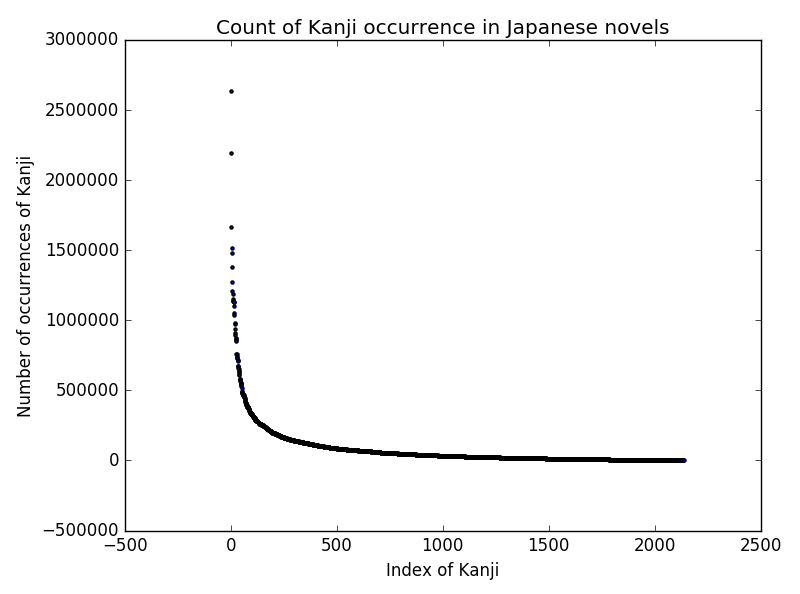
\includegraphics[width=0.9\linewidth]{Cap2/KanjiCountNovels}
    \caption{Linear distribution of Kanji.}
    \label{fig:linearkanjicount}
    \end{subfigure}
    \begin{subfigure}{0.475\textwidth}
    \centering
    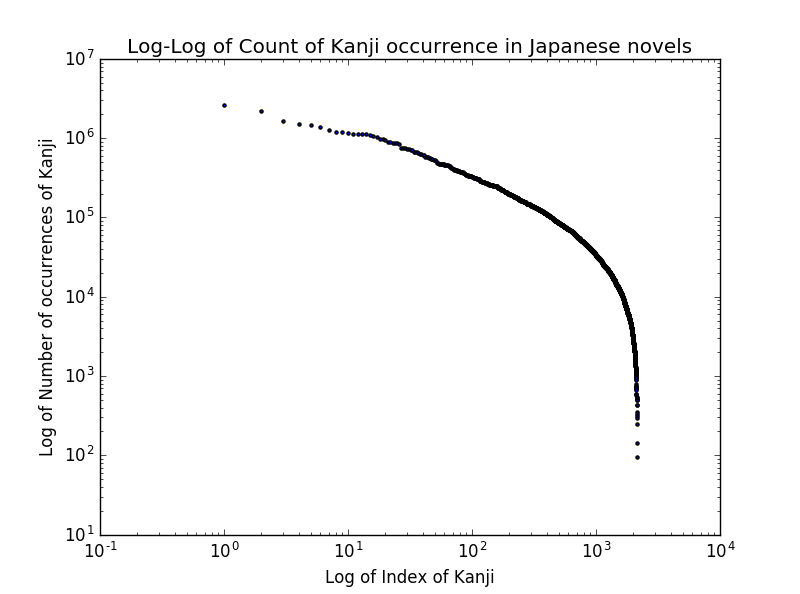
\includegraphics[width=0.9\linewidth]{Cap2/LogLogKanjiCountNovels}
    \caption{Log-Log of the distribution of Kanji.}
    \label{fig:logkanjicount}
    \end{subfigure}
    
    \caption{Distribution of Jouyou Kanji usage in Japanese Novels.}
    \label{fig:kanjicount}
\end{figure}

Once more, the linear graph is just auxiliary to the conclusion that a few of the elements concentrate most of the occurrences, but now we observe a smoother transition from the initial number of examples to the tail of the curve. This behaviour can be even more easily noticed in the Log-Log graph, where a curve that distances radically from a power log curve was created. In the specific case of Kanji, we note that the number of occurrences supports itself high even with an increase of rank from the Kanji approximately until the \(10^3\) mark. After this point, the distribution abruptly falls in number of occurrences for small logarithmic increments in the index.

This characteristic could be explained by the fact that the list of Jouyou Kanji was artificially created by the Ministry of Education in Japan, instead of forming over the pure necessity of users, as is the evolution process of a language and as it is still observer for general Japanese words. The Kanji chosen by the Japanese Government followed basically two rules, which could explain the two different sections of the occurrence graph:

\begin{enumerate}
    \item Kanji that represented frequently used concepts.
    \item Kanji that were already in use in legal documents from the government. This need arose from the strict rule that all public documents should be written exclusively with Jouyou Kanji. To accommodate this rule, Kanji that were obscure but were used in the legal jargon were introduced in the Jouyou Kanji list.
\end{enumerate}

To better elucidate this concentration of uses in a few Kanji, we generated an alternative view for this case. By dividing the number of occurrences by the total number of Kanji surveyed, we were able estimate the frequency of each Kanji as a fraction between 0 and 1. Furthermore, by adding each element with its previous frequency, we generated a cumulative distribution function of the use of Kanji. This CDF is presented in Figure \ref{fig:cdfkanji}.

\begin{figure}[hb]
    \centering
    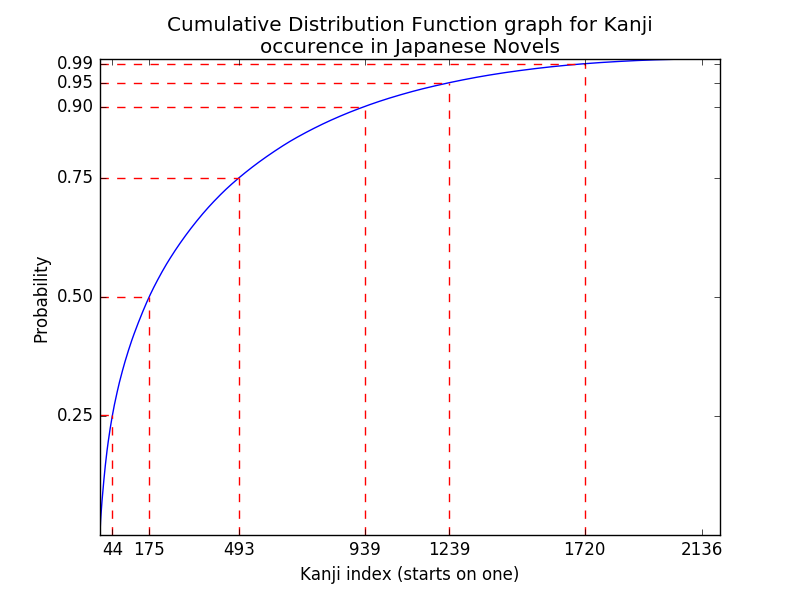
\includegraphics[width=0.8\linewidth]{Cap2/CDFKanji}
    \caption{Cumulative Distribution Function for the use of Jouyou Kanji in Japanese Novels}
    \label{fig:cdfkanji}
\end{figure}

The red references show the number of Kanji to be learned to reach some certain statistical level. As an example, it can be noted that 175 of the 2,136 Jouyou Kanji account for 50\% of the total occurrences of Jouyou Kanji in the surveyed novels. A deeper interpretation of this numbers will be presented on Section \ref{freqs:interpretation}.

\section{Comparing study efforts on pure frequency versus Kyouiku Kanji order}

As a base of reference, we will now proceed to study the distribution of the grades assigned by the Japanese Government for the Kyouiku Kanji list. Since no order is defined inside each of these six grades, we proceed to analyse the study of a student under the best-case scenario\footnote{although the student limits itself to proceed studying Kanji one grade at a time, he does so studying the most common Kanji first.} and the worst-case scenario\footnote{In this case, the student limits itself on the grades and study the least frequent Kanji first}. A representation of this curve on the best-case and worst-case scenarios is depicted in Figure \ref{fig:cdfgrade}.

\begin{figure}[ht]
    \centering
    \begin{subfigure}{0.9\textwidth}
    \centering
    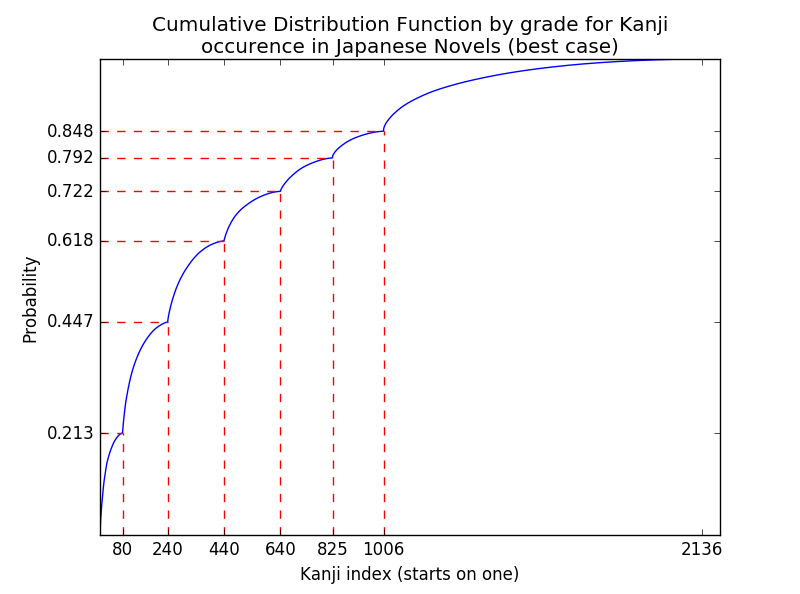
\includegraphics[width=\linewidth]{Cap2/CDFGrade}
    \caption{Best case scenario.}
    \label{fig:cdfgradebest}
    \end{subfigure}
    \begin{subfigure}{0.9\textwidth}
    \centering
    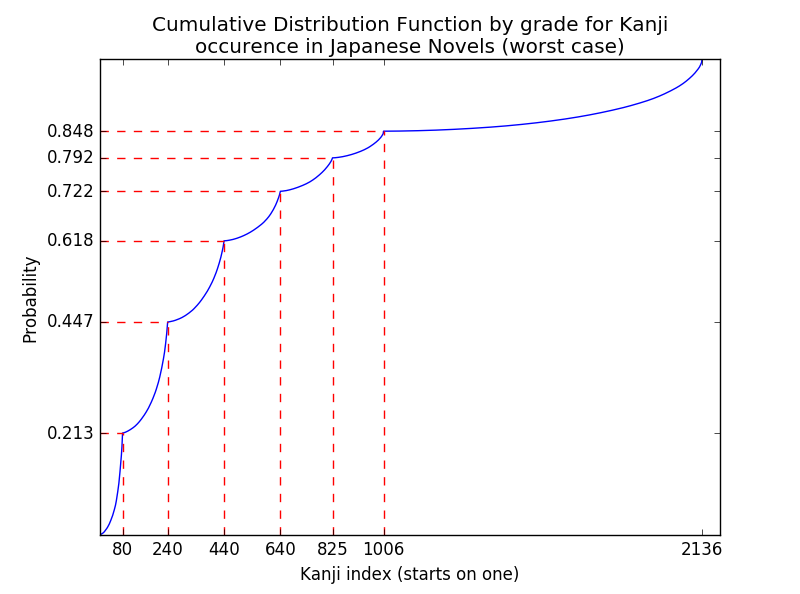
\includegraphics[width=\linewidth]{Cap2/CDFGradeWorst}
    \caption{Worst case scenario.}
    \label{fig:cdfgradebestworst}
    \end{subfigure}
    
    \caption{Cumulative Distribution Function limited by the grades determined in the Kyouiku Kanji.}
    \label{fig:cdfgrade}
\end{figure}

The reference lines in this case represent the number of Kanji to be studied in each grade and the corresponding expected value for the cumulative frequency up to that point. An example of this interpretation would be to state that after learning all the 1006 Kanji from primary school, a Japanese student is expected to recognize 84.8\% of the Kanji characters in a Japanese novel. As it could be expected, between the best and worst case scenarios the inflection points remain stable, representing the cumulative probability gain for each grade. The curves differ in each other inside grades and after the end of primary school in its concavity.

To better compare the study of a native Japanese following the grade lists and a student that uses the order implied by the relative frequencies of Kanji characters, those two curves were plotted together in Figure \ref{fig:cdfcomparison}, again separating in best and worst case scenarios.

\begin{figure}[ht]
    \centering
    \begin{subfigure}{0.9\textwidth}
    \centering
    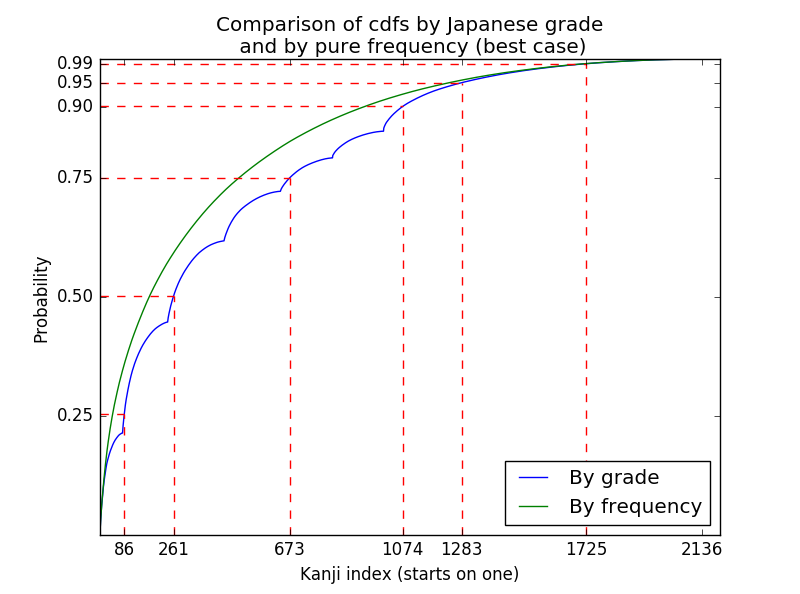
\includegraphics[width=\linewidth]{Cap2/CDFVersusGrade}
    \caption{Best case scenario.}
    \label{fig:cdfcomparisonbest}
    \end{subfigure}
    \begin{subfigure}{0.9\textwidth}
    \centering
    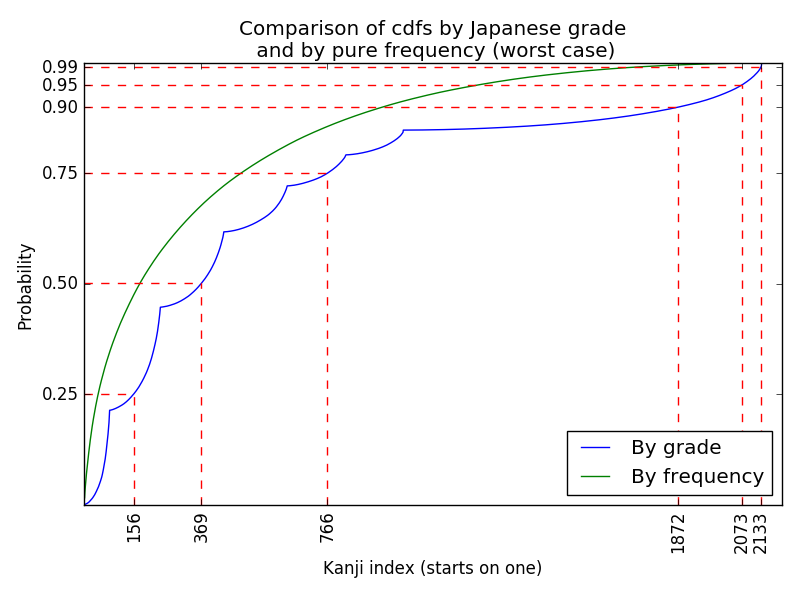
\includegraphics[width=\linewidth]{Cap2/CDFVersusGradeWorst}
    \caption{Worst case scenario.}
    \label{fig:cdfcomparisonworst}
    \end{subfigure}
    
    \caption{Comparison of the cumulative distribution functions bounded by grade and ordered solely through frequency.}
    \label{fig:cdfcomparison}
\end{figure}

In this case, the reference marks are used to depict the same reference probabilities as before, so that an effective comparison can be drawn between these two methods. The interpretation of these discrepancies are evaluated in the next Section.

\clearpage

\section{Kanji Probability Distribution Interpretation}\label{freqs:interpretation}

To better understand the information that can be drawn from these graphs, first we need to understand what does this cumulative probability distribution represents. An intuitive enunciation of the properties that follow from this analysis can be stated as follows:

\begin{center}
    "If I follow a certain strategy \textit{S} and have already studied \textit{N} Kanji, I'll have \textit{P} probability of having already studied a Kanji chosen arbitrarily in a random Japanese novel"
\end{center}

With this intuition, we can interpret the markings under the reference lines as the number of Kanji that should be studied if we want to know a certain percentage of characters that could be shown to us in a Japanese novel. A condensation of the information presented in Figures \ref{fig:cdfkanji} and \ref{fig:cdfcomparison} are put forward in Table \ref{tab:cdfcomparison}.

\begin{table}[ht]
\centering
\caption{Comparison of Kanjis to be studied to the same cumulative probabilities under different strategies}
\label{tab:cdfcomparison}
\begin{tabular}{|c|c|c|c|}
\hline
\multirow{2}{*}{\textbf{\begin{tabular}[c]{@{}c@{}}Probability of\\ having studied\end{tabular}}} & \multicolumn{3}{c|}{\textbf{Number of Kanji studied on Strategy}} \\ \cline{2-4} 
 & \textbf{Frequency} & \textbf{\begin{tabular}[c]{@{}c@{}}By Grades\\ (best case)\end{tabular}} & \textbf{\begin{tabular}[c]{@{}c@{}}By Grades\\ (worst case)\end{tabular}} \\ \hline
25\% & 44 & 86 & 156 \\ \hline
50\% & 175 & 261 & 369 \\ \hline
75\% & 493 & 673 & 766 \\ \hline
90\% & 939 & 1074 & 1872 \\ \hline
95\% & 1239 & 1283 & 2073 \\ \hline
99\% & 1720 & 1725 & 2133 \\ \hline
\end{tabular}
\end{table}

Firstly, we should appreciate the difference in proportions for the most efficient way of study by studying the first two columns of the table. For example, we note that by studying a total of 8.2\% (175) of the total number of Kanji we are already able to recognize half of all the Kanji occurrences in a Japanese novel. If we wish to be able to recognize 90\% of the Kanji, we only need to study a total of 44\% (939) of these. Furthermore, 99\% of occurrences are concentrated in 1,720 Kanji, leaving more than 400 Kanji sharing the last 1\% of occurrences. As we already commented in a previous Section, this distribution is not exactly Zipfian, but it does still follow a weak form of a Pareto rule, in a manner that an concentrated effort on the first few characters is much more justified than an indiscriminate study of Kanji.

By comparing columns two and three of Table \ref{tab:cdfcomparison}, we note that to reach 25\% of progress while following the Japanese grades but ordering them in the best case scenario, we will need to study roughly double the Kanji needed for the same probability in a study purely guided by frequency, which at this point are some measly 42 extra characters. This gap increases for 50\% and 75\% of probability, but closes down close to the end. This behaviour is attributable to the fact that that the last 1,133 are not divided in specific grades denominations, so that the gap between these two curves falls asymptotically after the inflection located at 84.8\% probability and 1,003 characters.

Now under the perspective of a unlucky student that follows the grade denominations but studies Kanji in the reverse order of their frequency, results are much more grim. To reach the mark of 25\% of probability of having studied an arbitrary character, this student needs to study 3.5 times more Kanji, or some extra 112 characters. This gap increases to almost 200 characters on 50\% probability, 273 for 75\%, 939 characters for 90\%, 834 characters for 95\% and 413 characters for 99\%. Note that at this point, the unlucky student would have studied 2,133 characters of the 2,136 total, leaving the last 1\% to be seen in the last three characters, a percentage that was dissipated among 416 characters in the best case.

A list with the ordered Kanji in decreasing frequency obtained from the data collected on this chapter is presented in the appendix, on Table \ref{tab:listfrequency}.

\chapter{Dealing With Kanji Readings}
\section{Motivation}
\subsection{Different Types of Readings}
\subsection{Why are there so many readings?}
\subsection{Relative Concentrations}
\section{Parsing Japanese Characters}
\subsection{Parallels to Compilers Theory}
\subsection{Brute Force Approach}
\subsection{Grammar Approach (TENTATIVE)}
\section{Enhancing Results Through Reading Types Labels}
\section{General Reading Distributions}
\section{Proportion of Regular to Irregular Kanji Use}

\chapter{Working With Graphs}
In the previous chapter we explored the concept of Kanji \textbf{importance}. In that point of the process, we associated the importance of a Kanji solely with its frequency in the Japanese language, in a way that more frequent Kanji are seem as more important than less frequent Kanji. In this chapter we will explore relations between Kanji to try and reach a more reasonable measure of importance.

There is in Computer Science a field of study that concerns itself with the study of mathematical structures that model pairwise relations between objects, the Graph Theory. In this chapter we will bring together our existent need to better rank the importance of Kanji with the existent solutions relative to Graph Theory.

\section{The PageRank Algorithm}
In 1998, Larry Page et al. published a paper that radically changed the scene for web search\cite{page1999pagerank}. In this paper they describe an algorithm devised to rank web pages objectively and mechanically, measuring the human interest and attention devoted to each page. In this paper they also compare the PageRank algorithm with an idealized random Web surfer, a comparison that will be useful for our application.

This algorithm estimates the rank of web pages based on the structure of hyperlinks that exist between t
hese pages. Figure \ref{fig:pagerank} shows an example graph and the solution to the ranking algorithm in this case.

\begin{figure}[ht]
    \centering
    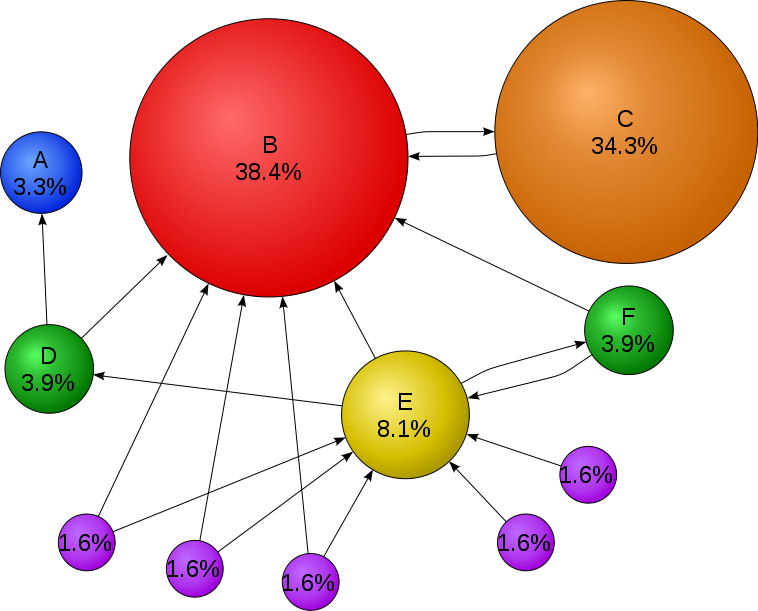
\includegraphics[width=0.75\linewidth]{Cap4/PageRankExample}
    \caption{Example of the ranking done by PageRank}
    \label{fig:pagerank}
\end{figure}

We can think of this algorithm as a flow for influence from pages, one that does not just count incoming links and outgoing links, but rather takes in consideration the influence of the page where this link is coming from, which is also calculated by this same algorithm, recursively. For example, in this graph we note that the rank for node "E" is smaller than the rank of node "C", even though the first has many more incoming links than the second. In this case, it can be seen that the pages that refer to "E" are of minor importance, while "C" is the only page hyperlinked from "B".

The second view that was described as useful for this algorithm is the random surfer abstraction. PageRank behaves as an estimate of the probability that of the node where the random surfer could be found in the graph after an arbitrary long time since the start starting from any node. His behavior would be to start at an arbitrary page on the web and than start a game of arbitrarily following hyperlinks to other pages. This representation allows us to find some problems that should be addressed at this point of the description, which are based on where the surfer can or can not go at any given point: the rank sinks.

\subsubsection{Dead Ends}
Let's firstly analyse dead ends, pages that have no outgoing link. At this point, our random surfer would get stuck in that page forever. That way, after a long enough time in the graph our imaginary surfer would get stuck in the dead end and the probability to find it there would be one (if only one such page existed). In the mathematical representation of this problem, it can be noted that the importance of the graph will "leak out" through such nodes, since those pages have no other pages to share its importance with. In the example picture, node "A" is a dead end.

\subsubsection{Spider Traps}
Spider traps are a similar kind of threat to our calculation, but it is more subtle one. Instead of being points where the user can't go anywhere else, spider traps are regions of the graph where the user would get stuck between pages from that region, with no outgoing links to other regions of the graph. One such case in the example Figure \ref{fig:pagerank} are nodes "B" and "C", that although both of them are not dead ends, once any user enters through "B" he would be stuck going back and forth between "B" and "C", and another case would happen if the "A" link had a link to itself. In these cases, all of the influence from the web would be drained by these regions.

\subsection{Random Teleports}
To solve this problem, Page et al.\cite{page1999pagerank} proposed the use of a vector parameter that would be responsible for random jumps in the graph. According to their description, the web surfer would get "bored" from time to time and jump to an arbitrary web page with probability $1-\beta$. Furthermore, in the case of dead end nodes the chance to jump to another random node would be one. 

\subsection{Non-Homogeneous Random Teleports}
Though this approach is sufficient for a basic rating of the web\footnote{Not that albeit this was the original algorithm for Google's search engine, many other papers were forwarded creating a better understanding of the topic, including an algorithm to counter-attack spam attempts: TrustRank}, it may be altered to be used for other objectives. This type of customization is commonly referred as Personalized PageRank, including by its creators\cite{page1999pagerank}. Although it is important to have random teleports to solve problems of dead ends and spider traps, there's no mathematical restriction that requires this teleport to be over \textbf{all} nodes of the graph or that this teleport should pick a jump node with equal probability for every node. The only requirement is that the jump probabilities make up for a total of 100\%.

One example of an application that personalizes the jump vector is the called Topic-Sensitive PageRank\cite{haveliwala2002topic}. This approach forces the random jump to be done to a page that is identified as being of a certain topic, so that the random restarts always come jump back not to any point of the web, but a very specific restart set. With this approach, it is possible to rank pages that are identified as being of a certain topic as well as pages that can be found after a small random walk from those pages.

This academic work focuses in another personalization of the jump vector: the non-homogeneous random teleports. In this approach, instead of giving an equal chance to all the nodes to be the targets of the random jump, we can skew the probabilities so that some nodes are more probable than others. For example, imagine a simple graph with three nodes. With homogeneous random restarts we would have a probability of $1/3$ to jumping to any node of the graph. If we use non-homogeneous random restarts however, it is possible to define a jump vector such as:
\[
\begin{bmatrix}
0.5 \\
0.3 \\
0.2
\end{bmatrix}
\]

With this application we can arbitrarily favour nodes in the graph as we see fit to the application at hand.

\subsection{Mathematical Representation}
Now that we've explained all the base intuition to the PageRank algorithm and the abstraction of the random web surfer, it is important that we also show the mathematical and computational base that can be used to implement these concepts.
\subsubsection{Flow Formulation}
Firstly, we can define mathematically the rank of a page $j$ as:
\[
r_j = \sum_{i \rightarrow j} \dfrac{r_i}{d_i}
\]
Where $j$ is a page, $i \rightarrow j$ represents all pages that point to $j$ and $d_i$ is the degree of $i$, measured as the number of outgoing links of $i$.
That is to say, the rank of a page j is the summation of the rank contributed by each of its incoming links, where each page contributes to the rank of each of its pointed pages by a fraction of its own rank and the number of pages it points. That being so, we consolidate our perspective that pages that point to many other pages will spread their influence among these, while pages that point to just a few will concentrate its influence on those. Note that since we start the process without knowing any of the ranks of the nodes, we end up with a system of $N$ variables and $N$ equations. To better solve this problem, we can condense all those equations in a matrix.

\subsubsection{Matrix Formulation}
The matrix that can be created to represent the mentioned flow equations is called an stochastic adjacency matrix. It is named as so because each column sums to 1 (since the outgoing link is spread evenly between its outgoing links). To illustrate this process and the resulting links, we introduce an example graph to be solved, which is presented in Figure \ref{fig:graphexample}.

\begin{figure}[ht]
    \centering
    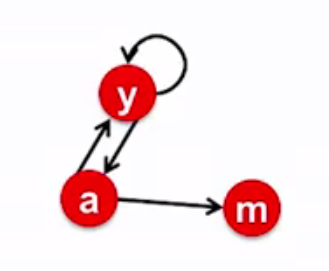
\includegraphics[width=0.4\linewidth]{Cap4/SmallGraph}
    \caption{An example of a small graph}
    \label{fig:graphexample}
\end{figure}

In this graph, we can write the flow equations as:
\begin{align*}
r_y &= \dfrac{1}{2}r_y + \dfrac{1}{2}r_a \\
r_a &= \dfrac{1}{2}r_y \\
r_m &= \dfrac{1}{2}r_a
\end{align*}
Note that at this point $r_m$ only appears once, since it is a dead end.

To turn this into a matrix we can write:
\[
\begin{bmatrix}
r_y \\
r_a \\
r_m
\end{bmatrix}
=
\begin{bmatrix}
1/2 & 1/2 & 0 \\
1/2 & 0 & 0 \\
0 & 1/2 & 0
\end{bmatrix}
\begin{bmatrix}
r_y \\
r_a \\
r_m
\end{bmatrix}
\]
That is, given that page $i$ has $d_i$ out-links, we set $M_ji=\dfrac{1}{d_i}$ if page $i$ points to page j, otherwise $M_ji=0$.

\subsubsection{Teleport Vector}
The matrix we've seen so far is similar to the Markov transition matrix. We can benefit from this proximity to use a result known for Markov chains:
\begin{center}
\textit
For any start vector, the power method applied to a Markov transition matrix \textbf{P} will converge to a unique positive stationary vector as long as \textbf{P} is stochastic, irreducible and aperiodic.\cite{pakes1969markov}
\end{center}
So, as discussed earlier, our transitions matrix can be made stochastic, irreducible and aperiodic by adding a stochastic column vector to all columns of this matrix\footnote{It is important to note that this can be any stochastic vector as long as all elements are different than zero. If some elements are equal to zero, we can not guarantee that the final matrix has these properties.}. Also, it is important that all columns that sum to zero (dead-ends) have 100\% probability to jump to a node from the restart set. If we use the homogeneous case we can do a pre-processing step to fix the $A$ matrix as:
\[
\begin{bmatrix}
1/2 & 1/2 & 0 \\
1/2 & 0 & 0 \\
0 & 1/2 & 0
\end{bmatrix}
\rightarrow
\begin{bmatrix}
1/2 & 1/2 & 1/3 \\
1/2 & 0 & 1/3 \\
0 & 1/2 & 1/3
\end{bmatrix}
\]
And also rewrite our base equation as:
\[
\begin{bmatrix}
r_y \\
r_a \\
r_m
\end{bmatrix}
=
\Bigg(
\beta \cdot
\begin{bmatrix}
1/2 & 1/2 & 1/3 \\
1/2 & 0 & 1/3 \\
0 & 1/2 & 1/3
\end{bmatrix}
+
(1-\beta) \cdot
\begin{bmatrix}
1/3 & 1/3 & 1/3 \\
1/3 & 1/3 & 1/3 \\
1/3 & 1/3 & 1/3
\end{bmatrix}
\Bigg)
\begin{bmatrix}
r_y \\
r_a \\
r_m
\end{bmatrix}
\]
If we now name the rank vector as $r$, our stochastic adjacency matrix as $M$ and the teleport matrix as $H$ we can rewrite the equation as:
\[
r = (\beta \cdot M + (1-\beta) \cdot H) \cdot r
\]
And we can proceed in naming $A = \beta \cdot M + (1-\beta) \cdot H$ to yield our final equation:
$$r = A \cdot r$$

\subsubsection{Solution Through Eigenvector calculation}
If we closely inspect the final equation for the PageRank calculation, we note that our equation in in the form
$$\lambda x = A \cdot x$$
that is, our equation represents the calculation of the eigenvector correspondent to the eigenvalue where $\lambda = 1$.

Since each column of $M$ sums to one and $r$ is a stochastic vector, we have that $Mr \leq 1$, so the sought after eigenvector is in fact the first or principal eigenvector. 

\subsubsection{Solution Through Power Iteration}
Although we could use a linear algebra package to solve our final equation, we have in hands a more efficient method to calculate a single eigenvector which has its eigenvalue known: the power iteration method. With this method, we start initializing $r^{(0)} = [1/N,...,1/N]^T$, and we iterate $r^{(t+1)} = M \cdot r^{(t)}$ as long as $|r^{(t+1)} - r^{(t)}|_1 > \epsilon$, where $|x|_1$ represents the $L_1$ norm of $x$\cite{arasu2002pagerank}.

Although other approaches designed to work at the scale of million of nodes exist, this method is efficient enough for the calculation of a problem as small as the determination of ranks of the 2,136 Jouyou Kanji.

\section{Modeling the study of Japanese Kanji as a PageRank Problem}
Well, now we know what to do, let's fetch some matrices!
\subsection{The Morphological Graph}
It exists cause they look like, are contained and contain each other.
Some examples.
\subsubsection{Creating the Morphological Graph}
By hand. Tragic.
Don't forget to speak about the frigging squares.
\subsubsection{Creation of the Relationships Matrix}
\subsubsection{Refining result to remove misc characters}
It is not just Jouyou Kanji that can be part of other Jouyou Kanji. Radicals, uncommons, Chinese only...

\subsection{The Co-occurrence Graph}
Words exist.
\subsection{Creating the Co-occurrence Graph}
\subsubsection{Creation of the Relationships Matrix}
\subsubsection{Managing occurrences with misc characters}

\section{Results}

\chapter{Applying Statistical Knowledge To Teaching Methods}
\section{Applications to Problems Related to Leveling Students}
\section{Modifying Spaced Repetition Models}
\section{Modelling User Interaction}
\section{Dangers of Gamefication Over-application}
\section{Multidimensional Flashcards}
\section{Reading Exercises}
\section{An Improved Kanji Search Tool Using Tries}

\chapter{Conclusion}
\input{Cap6/cap6}

% REFERENCIAS BIBLIOGRAFICAS
\renewcommand\bibname{\itareferencesnamebabel} %renomear título do capítulo referências
\bibliography{Referencias/referencias}

% Apendices
\appendix
\chapter{Placeholder for Appendix} %opcional
This annex serves to clarify technical terms and concepts from the field of linguistics that are relevant to the development of this academic project.

\section{Japanese as a Moraic System}\label{mora}
A Mora is a unit in phonology that can be defined as "something of which a long syllable consists of two and a short syllable consists of one"\cite{mccawley1968}. As per this definition, the Japanese is said to be moraic, since two of its base scripts (Hiragana and Katakana) translate strongly the concept of mora to its characters. 

For example, we can refer to the word \={O}saka, which could also be spelled as Oosaka (with a double "o") or in Hiragana \jap{おおさか}. This word would be be broken in three syllables: \={o}/sa/ka, but as denoted by the macron over the "o" letter, this is a long vowel. As can be seen in the Hiragana representation of this word, we have four graphemes, exactly the same as the number of morae. Though this is not always the case in Japanese, it is so in the great majority of cases, representing the importance of morae in the understanding of Japanese.

% Anexos
\annex
\chapter{Placeholder for Annex} %opcional
\section{Annex section placeholder}

% Glossario
%\itaglossary
%\printglossary

% Folha de Registro do Documento
% Valores dos campos do formulario
\FRDitadata{21 de Dezembro de 2016}
\FRDitadocnro{DCTA/ITA/TC-018/2016} %(o número de registro você solicita a biblioteca)
\FRDitaorgaointerno{Instituto Tecnológico de Aeronáutica -- Computer Engineering Division -- ITA}
%Exemplo no caso de pós-graduação: Instituto Tecnol{\'o}gico de Aeron{\'a}utica -- ITA

\FRDitapalavrasautor{Kanji; Language; Linguistics; Statistics; Pedagogy; Andragogy}
\FRDitapalavrasresult{Kanji; Language; Statistics}
%Exemplo no caso de graduação (TG):
\FRDitapalavraapresentacao{Trabalho de Graduação, ITA, São José dos Campos, 2016. \NumPenultimaPagina\ páginas.}
%Exemplo no caso de pós-graduação (msc, dsc):
%\FRDitapalavraapresentacao{ITA, São José dos Campos. Curso de Mestrado. Programa de Pós-Graduação em Engenharia Aeronáutica e Mecânica. Área de Sistemas Aeroespaciais e Mecatrônica. Orientador: Prof.~Dr. Adalberto Santos Dupont. Coorientadora: Prof$^\textnormal{a}$.~Dr$^\textnormal{a}$. Doralice Serra. Defesa em 05/03/2015. Publicada em 25/03/2015.}
\FRDitaresumo{TBD}
%  Primeiro Parametro: Nacional ou Internacional -- N/I
%  Segundo parametro: Ostensivo, Reservado, Confidencial ou Secreto -- O/R/C/S
\FRDitaOpcoes{N}{O}
% Cria o formulario
\itaFRD

\end{document}
% Fim do Documento. O massacre acabou!!! :-)
